\RequirePackage[l2tabu, orthodox]{nag}
\documentclass[11pt, a4paper, oneside, openright]{report}


\usepackage[left=30mm, right=20mm]{geometry}

\usepackage{microtype}
\usepackage{fixltx2e}

\usepackage{parskip}
\usepackage{titlesec}
%\usepackage[compact]{titlesec}

\usepackage[nottoc,notlof,notlot]{tocbibind}
\usepackage[sort,authoryear]{natbib}

\usepackage[pdftex]{graphicx}

\usepackage{flafter}
%\usepackage{float}
\usepackage{floatrow}
\floatsetup[table]{capposition=top}
\usepackage[titletoc,page]{appendix}
\usepackage[tableposition=top,width=.75\textwidth]{caption}
\usepackage{subcaption}

\usepackage{multirow}
\usepackage{booktabs}

\usepackage{amsfonts}
\usepackage{amsmath}
\usepackage{amssymb}
\usepackage{amsthm}
\usepackage{mathtools}

\usepackage{xcolor}
\usepackage{listings}
\usepackage{verbatim}
\usepackage{algorithm}
\usepackage{algorithmicx}
\usepackage[noend]{algpseudocode}


\usepackage{tikz}
\usetikzlibrary{shapes, arrows, calc}
\usepackage{pgfplots}

\setcounter{secnumdepth}{3}
\setcounter{tocdepth}{3}
%\setlength\parindent{0pt}

\setlength{\marginparwidth}{2cm}
\reversemarginpar

\lstset{
    language=C++, numbers=left, numberstyle=\tiny, stepnumber=1,
    frame=single, breaklines=true, showstringspaces=false, tabsize=4,
    commentstyle=\itshape\color{gray}, basicstyle=\footnotesize\ttfamily\bfseries, morekeywords={def}
}

\usepackage{url}
\usepackage{hyperref}

\hypersetup{
    colorlinks=false,
    pdfborder={0 0 0},
    pdftitle={Faster Shortest Path Computation for Traffic Assignment},
    pdfauthor={Boshen Chen}
}


\usepackage[draft, shadow, color=gray!15, linecolor=black]{todonotes} % final to turn off
\newcommand\todoin[2][]{\todo[inline, caption={2do}, #1]{ \begin{minipage}{\textwidth-4pt}#2\end{minipage}}}

\begin{document}

\thispagestyle{empty}
\setcounter{page}{0}
\pagenumbering{Alph}
\begin{titlepage}
    \newcommand{\HRule}{\rule{\linewidth}{0.5mm}}
    \centering
    
\includegraphics[width=0.5\textwidth]{img/logo.jpg}\\[2cm]    
    %\textsc{\LARGE University of Auckland}\\[1.5cm]
    \textsc{\Large Engineering Science}\\[2cm]
    \HRule \\[0.4cm]
    { \huge \bfseries Faster Shortest Path Computation for Traffic Assignment
    }\\[0.4cm]
    \HRule \\[2cm]

    \begin{minipage}{0.4\textwidth}
        \begin{flushleft} \large
            \emph{Author:}\\
            Boshen \textsc{Chen}
        \end{flushleft}
    \end{minipage}
    \begin{minipage}{0.4\textwidth}
        \begin{flushright} \large
            \emph{Supervisors:} \\
            Dr. Andrea \textsc{Raith} \\
            Olga \textsc{Perederieieva}
        \end{flushright}
    \end{minipage}\\[4cm]

    \vfill
    {\large \today}
    \thispagestyle{empty}
\end{titlepage} 

\pagenumbering{roman}

\newpage
\thispagestyle{empty}
\chapter*{Abstract}
The Traffic Assignment (TA) problem involves the selection of optimal path for every vehicle in a transportation network subject to congestion.
One method for solving TA is the Path Equilibration (PE) algorithm.
PE requires to find the shortest path repeatedly between every origin and destination pair in the network for a large number of iterations,
while the travel times of the roads change due to congestion.
The aim of this project is to find a faster shortest path algorithm for PE.
Dijkstra's algorithm, A* search and their bidirectional versions and eight different versions of priority queue data structures that improve these algorithms' performance are implemented.
Two strategies for skipping shortest paths altogether in the iterative environment of PE are also developed.
The first strategy is to avoid the next few iterations when the shortest path of the previous two iterations are the same.
The second strategy is to randomly skip the next shortest path calculation in the hope for the situation where the previous and current iteration is going to be the same.
We present experimental results that demonstrate the run time differences between the priority queues, shortest path algorithms and path calculation skipping strategies.
We conclude A* search algorithm using the priority queue implementation from the C++ standard template library with random skipping strategy has the best performance.

\thispagestyle{empty}
\begin{center}
\Huge Acknowledgements
\end{center}
I would like to thank my superviosrs, Dr Andrea Raith and Olga Perederieieva from the Department of Engineering Science at the University of Auckland,
for their patient guidance, assistance and useful critiques throughout this project.

I would also like to thank my fellow part IV students, especially Danny Tsai and Corey Kok, for their insightful ideas and kind helps, some of the algorithms would take much longer time to write without them.

Finally I would like to thank open-source software,
with out it bidirectional A* search would not have been written.



\setcounter{page}{3}

\renewcommand\contentsname{Table of Contents}
\tableofcontents 
\listoffigures
\listoftables
\listofalgorithms

\newpage
\pagenumbering{arabic}
\setcounter{page}{1}
\chapter{Introduction}
\section{Introduction to traffic modelling}
Nowadays a large portion of people's daily lives involve activities that relate to transportation.
For example, most people need to travel between their workplace and residence twice a day,
or buy goods from shops that need to be delivered across the city.
In the meanwhile, 
transportation networks expand and improve constantly to cater for people's demand for efficient travelling.
but the rate of improvement does not confront with the rate of population growth.
As a result,
the network becomes inefficient, resulting in traffic congestion.

Congestion leads to major economical losses due to time delays and increased usage of petrol.
Congestion causes air pollution that increases respiratory problems such as asthma, 
and the exhaust gas exacerbates global warming.
Congestion also increases noise pollution and causes frustration,
which in turn accelerates traffic accidents.
It is important for traffic designers to be able to reduce congestion problems,
and eliminate its negative effects.
%The transportation network can be improved by, for example,
%introducing road tolls to diverge traffic to less congested roads,
%or by educating people to use public transport.

Making improvements to the transportation network tends to be very costly,
so a good plan is necessary:
use the least amount of investment for the greatest change.
In order to make better plans for traffic design,
different mathematical models have been built to estimate the current and future behaviour of the transportation system.
One particular model called the transportation forecasting model is commonly used.
The aim of this model is to estimate future traffic usage when the system is changed.
For example, changes to a transport system can include upgrading or adding roads, changing roundabouts to traffic lights, or providing better public transport. 

The transportation forecasting model has 4 stages (shown in Figure~\ref{fig:model}):
trip generation, trip distribution, mode choice and traffic assignment \citep{Sheffi}.
In the model, the solution of each stage can be passed to the previous ones to improve transportation forecasting and traffic design.
This means the model can be calibrated numerous times to establish an accurate model which can estimate future traffic behaviour.
In summary, 
the model collects traffic demand data and 
generates origins and destinations for travellers (trip generation).
It then calculates the number of trips that are required between each origin and destination (trip distribution),
and decides which transportation method should be used for each trip (mode choice).
Finally it decides the route (e.g.\ the shortest path) that each trip needs to travel on (traffic assignment), 
where traffic flow is estimated for every modelled road in the network.
The traffic assignment problem in the last stage of the forecast model is a complicated problem.
This is because congestion occurs as traffic flows are assigned onto the network,
and it is very difficult to find an equilibrium situation where everybody in the network finds their best route.
Generally the equilibrium situation happens when it is assumed that people are selfish,
everyone tries to minimise travel times by travelling along their shortest paths.

\begin{figure}[!ht]
    \centering
    \tikzstyle{block} = [rectangle, draw, text width=10em, text centered, rounded corners, minimum height=2em]
    \tikzstyle{line} = [draw, -latex']
    \begin{tikzpicture}[node distance=4em]
        \node [block] (first) {Trip Generation};
        \node [block, below of=first] (second) {Trip Distribution};
        \node [block, below of=second] (third) {Mode Choice};
        \node [block, below of=third] (fourth) {Traffic Assignment};
        \path [line] (second) -- (third);
        \path [line] (first) -- (second);
        \path [line] (third) -- (fourth);
        \path [line] (fourth.west) -- ($(fourth.west)-(0.8,0)$) -- ($(first.west)-(0.8,0)$) -- (first.west);
        \path [line] ($(second.west)-(0.8,0)$) -- (second.west);
        \path [line] ($(third.west)-(0.8,0)$) -- (third.west);
    \end{tikzpicture}
    \caption{Transportation forecasting model}
    \label{fig:model}
\end{figure}

\section{Purpose of this project}
The transportation forecasting model has been implemented in many software packages for traffic design.
One key observation is that,
the traffic assignment problem can take hours, or even days to solve.
It turns out that,
the bottleneck is in the algorithm for solving the shortest path problem.
This is because algorithms for solving the traffic assignment problem are usually iterative,
where each iteration requires to find millions of shortest paths between every origin and destination in the network.
Although each shortest path calculation may take only a fraction of a second,
cumulatively the computational time can be very long.
Therefore the purpose of this project is to find a faster algorithm for solving the shortest path problem in an iterative environment.
As a result, traffic assignment will be solved faster
for larger and more complicated road networks.
This will also allow city designers to estimate traffic flows further into the future and make better decisions on road network design.

In summary,
The algorithms that are going to be studied are:
\begin{itemize}
    \item Bellman-Ford's label correcting algorithm,
    \item Dijkstra's label setting algorithm (using different data structures),
    \item Bidirectional Dijkstra's algorithm,
    \item A* search,
    \item Bidirectional A* search.
\end{itemize}

We also aim to find and discuss the following techniques that can speed up shortest path calculations in an iterative environment:
\begin{itemize}
    \item preprocessing algorithms,
    \item use information from the previous iterations,
    \item avoid shortest path calculations.
\end{itemize}

\section{Structure of the report}
Chapter~\ref{chap:ta} gives a short description of the traffic assignment problem
and presents a specific algorithm called the path equilibration algorithm that solves it.
This algorithm is the begin of our experiments for this project.
Chapter~\ref{chap:solvingspp} introduces the shortest path problem and presents some of the well established algorithms that solve it.
Implementation details are presented in Chapter~\ref{chap:implementation}.
%Strategies for solving the shortest path problem faster in an iterative environment are also described in this chapter.
Chapter~\ref{chap:results} shows the results and discussions for the algorithms described in Chapter~\ref{chap:solvingspp}.
Chapter~\ref{chap:iterative} presents strategies and results for solving the shortest path problem in path equilibration algorithm of the traffic assignment.
Finally conclusions and future work are drawn in Chapter~\ref{chap:conclusions}.


\newpage
\chapter{Solving the Shortest Path Problem}
\todo[inline]{do I need to show pseudocode for all algos?}
\label{chap:solvingspp}

Over the years,
various algorithms have been developed 
to address the problem of finding the shortest path in different situations.
In this chapter,
notations and definitions for the shortest path problem is stated first, 
the theory for solving the shortest path problem is described next,
algorithms that are applicable for road networks are then summarised,
including the discussion of their advantages and drawbacks.

\todo[inline]{Big O analysis for all algorithms}
\todo[inline]{Need to talk about results, what should the reader pay attention to? What should they conclude?}
\todo[inline]{assume a path always exist between an O-D pair}

\section{Notations and Definitions}
The Shortest Path Problem (SPP) is the problem of finding the shortest path from a given origin  to some destination.
There are two types of SPP hat are going to
be analysed in this chapter:
a single-source and a point to point SPP.  
The Frank-Wolfe algorithm in the TA involves
solving the single-source SPP by finding of shortest path going from one origin to every other destinations the network.
The Path Equilibration method in the TA
Solving the point to point SPP solves from one origin to a specific destination and is used in the Path Equilibration method. 

When solving SPP for a normal road network,
different measurements such as distance and travel exist for the road length.
But in traffic assignment,
the road length is measured in a non-decreasing travel time function,
which encapsulates information such as traffic flow, road capacity and travel speed.
This travel time function is always non-negative so taking advantage of this helps the selection of algorithms that uses this property.
\todo{show equation?}

Using notations from \citet{Cormen} and \citet{Klunder} and in the context
of transportation networks,
we denote $ G = ( V, E ) $ for a weighted, directed graph,
where $ V $ denotes the set of nodes (origins, destinations, and intersections)
and $ E $ the set of edges (roads);
we say $ E $ is a subset of the set $ \{ (u, v)\, | \, u, v \in V \} $ of all ordered pairs of nodes.
We denote the weight function $ c : E \rightarrow \mathbb{R} $ which assigns a cost (travel time) to any arc $ (u,v) \in E $.
We write the costs of arc $(u, v)$ as: $ c((u, v)) = c_{uv} $.

The path $P$ inside a transportation network has to be a directed simple path, 
which is a sequence of nodes and edges $ (u_1, (u_1, u_2), u_2, \ldots , (u_{k-1}, u_k), u_k ) $
such that $ (u_i, u_{i+1}) \in E$ for $i = 1,\ldots,k-1$ and $u_i \neq u_j$ for all $ 1 \leq i < j \leq k$.
Note $u_1$ is the origin and $u_k$ is the destination of the path $P$, $u_1$ and $u_k$ together is called an O-D pair for this path.
For simplicity, we denote $s$ to be the source (origin) and $t$ to be the target (destination) for any path $P$.
%Finally we denote cost of the whole path $C(P) := \sum_{(u,v)\in P} c_{vw}$.

In a transportation network,
the origins and destinations are often called centroids or zones.
They are traffic analysis zones for generating trip demands and supplies
and hold information such as household income and employment information,
these information helps the understanding of trips that are produced and attracted within the zone.
The zones are conceptual nodes in the network and are untravellable,
which means a path between two zone nodes must not contain another zone node.
\todo[inline]{Maybe a picture of the network explain what the zones are.}

Through out the report,
run-time analysis (big O and other notations) is used to demonstrate the estimation of algorithms running time regarding their input size. 
\todo[inline]{How do I nicely say `let the reader refer to other resources?'
or do I desribe what big O notation is?}

\section{Generic Shortest Path Algorithm}
A family of algorithms exist for solving SPP with directed non-negative length edges,
in this section we describe the generic case for these
algorithms, the generic shorest path algorithm (GSP).

This family of algorithms aim at finding a 
vector ($d_1, d_2,\dots d_v$) of distance labels and its corresponding shortest path \citep{Klunder}.
Each $d_v$ keeps the least distance of any path going from $s$ to $v$, $d_v = \infty$ if no paths has been found.
A shortest path is optimal when it satisfies the following conditions:
\begin{align}
    d_v \leq d_u + c_{uv}, \quad \forall(u,v) \in E, \label{eq:Bellman1}\\
    d_v  =   d_u + c_{uv}, \quad \forall(u,v) \in P.
\end{align}
\todo[noline]{what is $P$?}
The inequalities~(\ref{eq:Bellman1}) is called Bellman's condition \citep{Bellman}.
In other words,
we wish to find a label vector $d$ which satisfies Bellman's condition for all of the vertices in the graph.
To maintain the label vector, the algorithm uses a queue $\mathcal{Q}$ to store the label distances.

In the label vector,
a node is said to be unvisited when $d_u = \infty$,
scanned when $d_u \neq \infty$ and is still in the queue,
and labelled when the node has been retrieved from the queue and its distance label cannot be updated further.
If a node is labelled then its distance value is guaranteed to represent the minimal distance from $s$ to $t$, Bellman's condition must have been satisfied.

In the generic shortest path algorithm,
we start by putting the origin node in the queue,
and then iteratively find the arc that violates the Bellman's condition (i.e., $d_v > d_u + c_{uv}$),
distance labels are set to a value which satisfies condition (\ref{eq:Bellman1}) to the corresponding node of that arc.
Shortest path going from $s$ to all other nodes in $V$ is found when (\ref{eq:Bellman1}) is satisfied for all edges in $E$.
It may not be obvious but negative costs are permitted in the GSP but not negative cost cycles.

We use $p_u$ to denote the predecessor of node $u$.
The shortest path can be constructed by following the predecessor of the destination node $t$ back to the origin node $s$. $p_s$ is often set to $-1$ to indicate it does not have a predecessor.

\todo[inline]{diagram showing $u, v, c_{vw}$ etc.}

Algorithm~\ref{algo:gsp} \citep{Klunder} describes the generic shortest path algorithm mentioned above,
with an extra constraint required when solving a TA problem: travelling through zone nodes are not permitted.
In essence, this algorithm repeatedly selects node $u\in\mathcal{Q}$ and checks the violation of Bellman's condition for all emanating edges of node $u$.
\begin{algorithm}
    \caption{The Generic Shortest Path Algorithm}
    \label{algo:gsp}
    \begin{algorithmic}[1]
        \Procedure{GenericShortestPath}{$s$}
        \State $\mathcal{Q} \gets \mathcal{Q} \cup \{s\}$ \Comment{initialise queue with source node}
        \State $p_s \gets -1$ \Comment{origin has no predecessor}
        \State $d_s \gets 0$
        \ForAll {$ u \in V : u \neq s $} \Comment{all nodes are unvisited except the source}
        \State $d_u \gets \infty$
    \EndFor

    \While{ $\mathcal{Q} \neq \emptyset$ }
    \State $ u \gets \text{next}(\mathcal{Q}) $ \Comment{select next node}
    \State $ \mathcal{Q} \gets \mathcal{Q} \setminus \{u\} $
    \If{ $u \neq \text{zone} $}
    \ForAll {$v : (u, v) \in E$} \Comment{check Bellman's condition for all successors of $u$}
    \If {$d_u + c_{vw} < d_v$}
    \State $d_v \gets d_u + c_{vw}$
    \State $p_v \gets u$
    \If {$v \notin \mathcal{Q}$} 
    \State $\mathcal{Q} \gets \mathcal{Q} \cup \{v\}$ \Comment{add node $v$ to queue if unvisited}
\EndIf
                    \EndIf
                \EndFor
            \EndIf
        \EndWhile
    \EndProcedure
\end{algorithmic}
\end{algorithm}

Algorithm~\ref{algo:gsp} is generic because of two reasons:
the rule for selecting the next node $u$ (the next function in line 8) and
the implementation for the queue $\mathcal{Q}$ is unspecified.
Different algorithms use different rules and implementations to give 
either the one-source or the point-to-point shortest path algorithm \citep{mplomer}.
The next two sections describes these rules and implementations.

\section{Label Correcting Algorithm}
\todo[inline]{pseudo code}
\label{section:labelcorrectingalgorithm}
The GSP is addressed as a label correcting algorithm when the queue is a first in first out (FIFO) queue.
\todo{Check if its FIFO or double ended queue}
Given the arc costs can be negative in the GSP,
and in order to satisfy the Bellman's conditions for all edges,
the algorithm has to scan all edges $|V|-1$ times,
giving a run time of $O(|V||E|)$.

In this algorithm,
the distance labels do not get permanently labelled when the next node in the queue is retrieved,
another node may `correct' this node's distance label again,
thus the name label correcting algorithm.
This algorithm is also called the Bellman–Ford–Moore algorithm credited to \citet{Bellman, Ford} and \citet{Moore}.

\section{Label Setting Algorithm}
\label{section:labelsettingalgorithm}
The classical algorithm for solving the single-source shortest path problem is the label setting algorithm published by \citet{Dijkstra}.
The algorithm is addressed as label setting because when the next node $u$ is retrieved from the queue,
it gets permanently labelled;
the shortest path going to this node is solved and 
the distance label represents the shortest length.
In order to achieve label setting, 
the queue $\mathcal{Q}$ is modified to always have the minimum distance label in front of the queue,
hence the algorithm iterates through every node in the graph exactly once,
labelling the next node $u$ in the order of non-decreasing distance labels.

The advantage of this algorithm over the label correcting algorithm is
that all nodes in the graph are only visited once;
the shortest path tree grows radially outward from the source node.
It is clear that when the next node in the queue is the destination node,
the algorithm can be stopped for the point to point SPP case,
which is desirable for the Path Equilibration method.

\subsection{Priority Queue Implementations}
The run time performance of Dijkstra's algorithm depends heavily on the implementation of the queue for storing the scanned nodes,
\citet{Cormen} suggest the use of a min-priority queues.
Min-priority queues are a collection of data structures that always serve elements with higher priorities. The priority in SPP are the distance labels:
smaller distance label have a higher priority.

Algorithm~\ref{algo:p2pdijkstra} shows the use of the min-priority queue in Dijkstra's algorithm.
The min-priority queue has 3 main operations: Insert, Extract-Min and Decrease-Key.
The Insert operation (line $2$ and $17$ in Algorithm~\ref{algo:p2pdijkstra}) is used for adding new nodes to the queue, the Extract-Min operation (line 8) is used for getting the element with the minimum distance label and the Decrease-Key is used for updating the distance if the node is already in the queue.

\begin{algorithm}[H]
    \caption{Point to Point Dijkstra's Algorithm}
    \label{algo:p2pdijkstra}
    \begin{algorithmic}[1]
        \Procedure{Dijkstra}{$s, t$}
        \State $\text{Insert}(\mathcal{Q}\text{ , u})$ \Comment{initialise priority queue with source node}
        \State $p_s \gets -1$ \Comment{origin has no predecessor}
        \State $d_s \gets 0$
        \ForAll {$ u \in V : u \neq s $} \Comment{all nodes are unvisited except the source}
        \State $d_u \gets \infty$
    \EndFor

    \While{ $\mathcal{Q} \neq \emptyset$ }
    \State $ u \gets \text{Extract-Min}(\mathcal{Q}) $ \Comment{select next node with minimum value}
    \If{ u = t}
    \State $\text{Terminate Procedure}$ \Comment{finish if next node is the destination}
\EndIf
\If{ $u \neq \text{zone} $}
\ForAll {$v : (u, v) \in E$} \Comment{check Bellman's condition for all successors of $u$}
\If {$d_u + c_{vw} < d_v$}
\State $d_v \gets d_u + c_{vw}$
\State $p_v \gets u$
\If {$v \notin \mathcal{Q}$} 
\State $\text{Insert}(\mathcal{Q}, v)$ \Comment{add node $v$ to queue if unvisited}
\Else
\State $\text{Decrease-Key}(\mathcal{Q}, v)$ \Comment{else update value of $v$ in queue}
    \EndIf
\EndIf
                \EndFor
            \EndIf
        \EndWhile
    \EndProcedure
\end{algorithmic}
\end{algorithm}

According to \citet{Cormen},
a min-priority queue can implemented via an array or a binary min-heap, where each implementation give different run time performances.

In the array implementation,
the distance labels are stored in an array where the $n^{\text{th}}$ position gives the distance value for node $n$.
Each Insert and Decrease-Key operation in this implementation takes $O(1)$ time, and each Extract-Min takes $O(|V|)$ time (searching through the entire array), giving a overall time of $O(|V|^2 + |E|)$.

A binary min-heap is a binary tree which satisfies the min-heap property:
the value of each node is smaller or equal to the value of its child nodes.
\citet{Cormen} shows that if the graph is sufficiently sparse (in particular $E = o(|V|^2/\log(|V|))$, Dijkstra's algorithm can be improved with a binary min-heap. In this implementation, the binary tree takes $O(|V|)$ time, Extract-Min takes $O(\log(|V|))$ time for $|V|$ operations and Decrease-Key takes $O(\log(|V|))$ time for each $|E|$. The total running time is therefore $O((|V|+|E|)\log(|V|))$, which improves the array implementation.

The running time can be improved further using a Fibonacci heap
developed by \citet{Fredman}.
Where historically, the development of Fibonacci heaps was motivated by the observation that Dijkstra's algorithm typically makes many more Decrease-Key calls than Extract-Min.
In Fibonacci heap, each of the $|V|$ Extract-Min operations take $O(\log(V))$ amortized time,
and each of the $|E|$ Decrease-Key operations take only $O(1)$ amortized time,
which gives a total running time of $O(V\log(V)+E)$.

Min-priority queue can also be implemented as a binary search tree,
where the worst case for insertion, deletion and search for an element in the tree all run in $O(log(n))$ time.
Dijkstra's algorithm (Algorithm~\ref{algo:p2pdijkstra}) can be modified for a binary search tree implementation: when a label distance of node can be updated, we remove that node from the tree and insert a new one with the update value, which is analogous to the Decrease-Key operation.
Dijkstra's algorithm using a binary search also runs $O((|V|+|E|)\log(|V|))$ in the worst case compared to the min-binary heap.
The advantage of using a binary search tree is that we do not have to keep track of information about whether a node is in the queue,
since we just delete the node from the tree and add the node with a different value, and there is no harm deleting a non-existent node from the tree.

\section{Bidirectional Label Setting Algorithm} \label{section:bidirectional}
Dijkstra's algorithm can be imagined to be searching radially outward like a circle with the origin in the centre and destination on the boundary.
Likewise, Dijkstra's algorithm can be used on the reverse graph (all edges reversed in the graph) from the destination node.
Thus Dijkstra's algorithm can be run on the origin and destination simultaneously at the same time.
The motivation for doing this is because the number of scanned nodes can be reduced when searching bidirectionally:
two smaller circles growing outward radially instead of a larger one.
\todo{illustrate this}
It is common to conclude that the shortest path is found when the two searches meet somewhere in the middle,
but this is not actually the case.
There may exist another arc connecting the two frontiers of the searches that has a shorter path.
\todo{show proof?}
The correct termination criteria was first designed and implementation by \citet{Pohl} based on researches presented by \citet{Dantzig, Nicholson} and \citet{Dreyfus}.
\citet{Klunder} summarises the procedure and algorithm (Algorithm~\ref{algo:bidirectional}) for the termination criteria presented by \citet{Pohl}.

In Algorithm~\ref{algo:bidirectional},
two independent Dijkstra's algorithms are alternatively run on the forward  and reverse graph (forward and backward algorithm),
the algorithms terminate when a node is permanently labelled in both directions.
Once the algorithms have terminated,
the correct shortest path is found by looking for a arc connecting the frontiers of the two searches that may yield a shorter path.
This extra condition increases the run time significantly, 
searches have to be done for all edges that connect all labelled nodes in the forward search to all labelled nodes in the backward search.
\todo{Show theorem and proof?}

Note in Algorithm~\ref{algo:bidirectional},
$\mathcal{R}^s$ is the subset of nodes that are permanently labelled from $s$ with labels $d_v^s$ in the forward search, and 
$\mathcal{R}^t$ is the subset of nodes that are permanently labelled from $s$ with labels $d_v^t$ in the backward search.

\begin{algorithm}[H]
    \caption{Bidirectional Label Setting Algorithm }
    \label{algo:bidirectional}
    \begin{algorithmic}[1]
        \Procedure{Bidirectional}{$s, t$}
        \State Execute one iteration of the forward algorithm.
        If the next node $u$ is labelled permanently by the 
        backward algorithm $(u\in\mathcal{R}^t)$, go to step 3.
        Else, go to step 2.
        \State Execute one iteration of the backward algorithm.
        If the next node $u$ is labelled permanently by the
        forward algorithm $(u\in\mathcal{R}^s)$, go to step 3.
        Else, goto step 1.
        \State Find $\min\{\min\{d_v^s + c_{vw} + d_w^t | v \in \mathcal{R}^s, w \in \mathcal{R}^t, (v, w) \in E\}, d_u^s + d_u^t\}$, which gives the correct shortest path between $s$ and $t$.
    \EndProcedure
\end{algorithmic}
\end{algorithm}

In recent years,
\citet{Goldberg05} improved the bidirectional algorithm using a better termination condition,
where step 3 of Algorithm~\ref{algo:bidirectional} is embed during the searches.
The termination condition is summarized as the following.
During the forward and backward search,
we maintain the length of the shortest path seen so far, $\mu$, and its corresponding path. Initially, $\mu = \infty$.
When an arc $(v,w)$ is scanned by the forward search and $w$ has already been scanned in the reverse search (or vice versa),
we know the shortest $s-v$ and $w-t$ path have lengths $d_v^s$ and $d_w^t$ respectively.
If $\mu > d_v^s + c_{vw} + d_w^t$ then this path is shorter than the one detected before, 
so we update $u$ and its path accordingly.
The algorithm terminates when the search in one direction selects a node already scanned in the other direction.

\citet{GoldbergEPP} showed and proved a stronger termination condition on top of his previous one.
The searches can be stopped if the sum of the top priority queue values is greater than $\mu$:
\[
    \text{top}_f + \text{top}_r \geq \mu
\]
where $\text{top}_f$ and $\text{top}_r$ are the top priority queue values in the forward and reverse search, they the next minimum distance label that have not been labelled.
\todo{Show theorem and proof as well?}

\section{A* Search}
Up until now,
Dijkstra's algorithm does not take into account the location of the destination,
the shortest path tree is grown out radially until the destination is labelled.
In a traditional graph where actual distances are used for the distance labels,
a heuristic can be used to direct the shortest path tree to grow toward the destination (an ellipsoid in stead of a circle).
\todo{show figure}
If the heuristic estimate is the distance from each node to the destination,
and the estimate is smaller than or equal to the actual distance going to that destination,
then a shortest path can be found. This is called A* search or goad directed search, first described by \citet{Astar}.

Formally we define the following.
Let $h_v$ be a heuristic estimate from node $v$ to destination $t$,
and apply Bellman's condition such that an optimal solution exist, that is 
\begin{align}
    &h_v \leq h_u + c_{uv} \quad \forall(u,v) \in E, \\
    &h(t) = 0,
\end{align}
where $t$ is the destination node.
This means the heuristic function $h$ must be admissible and consistent.
The heuristic must never overestimate the actual path length and the estimated cost of a node reaching its destination node must not be greater than the estimated cost of its predecessors.
Note a consistent heuristic is also admissible but not the opposite.
\citet{Astar} proves if the heuristic function (such as using geographical coordinates and Euclidean distance) is admissible and consistent,
then A* is guaranteed to find the correct shortest path with a better time performance by scanning less nodes and edges.

To implement A* search,
Dijkstra's algorithm is modified.
Instead of selecting the node with the minimum distance label in the priority queue,
we select the next node $u$ that has the minimum distance label added with the heuristic value, which is $d_u + h_{ut}$ where $h_{ut}$ is the estimated distance from node $u$ to destination $t$.

In the Path Equilibration method,
geographical coordinates and Euclidean distances can not be used for the heuristic estimate because a travel time function is used for the length of the edges.
Instead, zero-flow travel time from every node to the destination can be used for the heuristic.
Zero-flow travel time admissible and consistent and can be shown by
analysing the travel times function (Figure~\ref{fig:flowfunction}).
The travel times function is a non-decreasing function with the lowest value being the zero-flow travel times.
This means using zero-flow travel times as the heuristic estimate
is assured to be admissible
as no travel time can be lower than the zero flow travel at any time.
The heuristic function is consistent because the travel time from a node to the destination must be no longer than all its predecessors.

\begin{figure}[H]
    \centering
    \missingfigure[figwidth=\textwidth]{Travel time function}
    %\begin{tikzpicture}
    %    \begin{axis}
    %        [
    %            domain=0:2500,
    %            black, no markers, smooth,
    %        %xtick=\empty, ytick=\empty,
    %            xlabel=flow(vehicles per hour), ylabel=travel time (hours),
    %            xmin=0,xmax=2500,
    %            ymin=0.16,ymax=0.2,
    %            yticklabel style={/pgf/number format/fixed, /pgf/number format/precision=3}
    %        ]
    %        \addplot {0.166*(1+0.15*(x/2000)^5)}; 
    %    \end{axis}
    %\end{tikzpicture}
    \caption{Travel time function.}
    \label{fig:flowfunction}
\end{figure}

\begin{comment}
\subsection{Linear Programming Perspective}
\todo[inline]{incomplete}
A* search can be describe in a linear programming perspective.
The reduced cost is $c_{ij} - y_j +y_i$ where $y_j$ and $y_i$ are the dual variables for $(i,j) \in E$, 
essentially A* search puts weight on the edges to and select  out the path with the maximum reduces cost, the weight is the heuristic values.
\begin{alignat}{2}
    \text{Primal: Minimise}   & \quad \sum_{(i, j)\in E} c_{ij} x_{ij} \\
    \text{Subject to} & \quad \sum_j x_{ij} - \sum_j x_{ji} = 0 \quad \forall i\\
    & \quad \sum_j x_{sj} - \sum_j x_{js} = 1 \\
    & \quad \sum_j x_{tj} - \sum_j x_{jt} = -1 \\
    & \quad x_{ij} = \{0,1\} \quad \forall (i,j) \in E
\end{alignat}

\begin{alignat}{2}
    \text{Dual: Maximise} & \quad y_t - y_s \\
    \text{Subject to} & \quad y_j - y_i \leq c_{ij} \quad \forall (i,j) \in E \\
    \text{where} & \quad y_{\cdot} = \sum_j x_{\cdot j} - \sum_j x_{j\cdot}  
\end{alignat}
\end{comment}

\section{Bidirectional A* Search}
Bidirectional search can also be applied to A* search,
where two ellipsoids are extended from the origin and destination respectively.
One may construct the shortest path with the same termination condition described in section~\ref{section:bidirectional}.
But this would not work.
This is due to fact that A* search does not label the nodes permanently in the order of their distance from the origin \citep{Klunder},
the heuristic estimations are no longer consistent.

The strategy for the correct use of heuristic estimates and termination criterion has first been published by \citet{Pohl}. The use of heuristic estimates is later improvement by \citet{Ikeda} and the termination criterion is improved by \citet{GoldbergEPP}.

The strategy is as follows. The heuristic estimates need to translated to consistent functions first. 
We denote $\pi_f(v)$ the estimate on distance from node $v$ to the destination $t$ in the forward search and $\pi_r(v)$ the estimate on distance from origin $s$ to node $v$ in the backward (reverse) search.
\todo{illustrate!}
In general two arbitrary feasible functions $\pi_f$ and $\pi_r$ are not consistent, but their average is both feasible and consistent \citep{Ikeda}:
\begin{align}
    p_f(v) = \frac{1}{2}(\pi_f(v)-\pi_r(v)) + \frac{\pi_r(t)}{2} \\
    p_r(v) = \frac{1}{2}(\pi_r(v)-\pi_f(v)) + \frac{\pi_f(s)}{2} 
\end{align}
where the two constants $\frac{\pi_r(t)}{2}$ and $\frac{\pi_f(s)}{2}$ are added by \citet{GoldbergEPP} to provide better estimates.
Note the modified consistent heuristic $p$ provides worse bounds than the original $\pi$ values.

Finally \citet{GoldbergEPP} shows and proves the stopping criterion:
\begin{align}
    \text{top}_f + \text{top}_r \geq \mu + p_r(t),
\end{align}
where is $\mu$ the best $s-t$ path seen fast, $\text{top}_f$ the length of the path from $s$ to the top node (minimum distance label) in the forward search priority queue and $\text{top}_r$ the length of the path from $t$ to the top node in the backward search priority queue.

\section{Preprocessing and More}
\todo[inline]{this section is in draft stage}
Preprocessing - trade memory to get faster time.
We can either do a fast preprocessing between iterations to make query in each iteration (so combined speed is still faster) 
or do a long preprocessing at the start and use the computed heuristic values
\begin{itemize}
    \item A* landmarks and triangle inequality (ALT)
    \item Reach-based routing 
    \item ALT + Reach
    \item Geometric Containers
    \item Arc Flags
\end{itemize}

If we have more data on the network we can use
algorithms that use hierarchies.
Consider roads with higher speed first: use a hierarchy of subgraphs.
\begin{itemize}
    \item Radius search.
    \item multi-level approach
    \item highway hierarchies
\end{itemize}

\todo[inline]{Extract from: Speed-Up Techniques for Shortest-Path Computations by Dorothea Wagner, Thomas Willhalm, and Fast Shortest Path Algorithms for Large Road Networks by Faramroze Engineer }

We can also try Lifelong Planning A* (LPA*), using heuristic from previous each iteration, but the original paper says only a few percent arc change can boost run time, not idea if it is more than that. 

If the edge lengths are whole numbers then we can use multi-level bucket for the priority queue.




\newpage
\chapter{Solving the Shortest Path Problem}
\label{chapter:solvingspp}

In this chapter we solve the shortest path problem
for transportation networks and sequentially
improve the existing algorithm implemented.
Run time improvement is then shown and discussed.

\marginpar{TODO}
{
    TODO: run time (Big O) analysis for all algorithms.
}
\section{General Shortest Path Algorithm}
Most algorithms for SPP depend on solving a label vector ($d_1, d_2,\dots d_v$).

Each $d_v$ keeps the least distance of of any path going from $s$ to $v$, $d_v = \infty$ if no paths has been found.
A shortest path is optimal when it satisfies the Bellman's conditions:
\begin{align}
    d_v \leq d_u + c_{uv}, \quad \forall(u,v) \in \mathcal{A}, \label{eq:Bellman1}\\
    d_v  =   d_u + c_{uv}, \quad \forall(u,v) \in \mathcal{P}.
\end{align}
\marginpar{Bellman's\\conditions}
In other words,
we wish to find a label vector $d$ which satisfy the Bellman's conditions for all of the vertices in the graph.
To maintain the label vector, the algorithm uses a candidate list $\mathcal{Q}$ to store the label distances.
A node is said to be unvisited when $d_u = \infty$,
scanned when $d_u \neq \infty$ and is still in the candidate list,
and labelled when the node has been retrieved from the candidate list and its distance label cannot be updated further.
In the general shortest path algorithm,
we start by putting the origin node in the queue,
and then iteratively find the arc that violates the Bellman's condition (i.e., $d_v > d_u + c_{uv}$),
distance labels are set to a value which satisfy condition (\ref{eq:Bellman1}) to the corresponding node of that arc.
Shortest path going from $s$ to all other nodes in $\mathcal{V}$ is found when (\ref{eq:Bellman1}) is satisfied for all arcs in $\mathcal{A}$.
We use $p_u$ to denote the predecessor of node $u$;
shortest path can be constructed by following the predecessor of destination node $t$ back to origin node $s$.
\marginpar{TODO}

{
    TODO:
    add diagram showing $u, v, c_{uv}$ etc.?
}

The following pseudo code describes the generic shortest path (GSP) algorithm mentioned above,
with an extra constraint than a normal GSP: travelling through zone nodes are not allowed.
\begin{algorithm}
    \caption{The General Shortest Path Algorithm \citep{Klunder}}
    \begin{algorithmic}[1]
        \Procedure{GeneralShortestPath}{$s$}
        \State $\mathcal{Q} \cup \{s\}$ \Comment{Initialisation}
        \State $p_s \gets -1$
        \State $d_s \gets 0$
        \ForAll {$ u \in \mathcal{V} : u \neq s $} \Comment{All nodes unvisited except the source}
            \State $d_u \gets \infty$
        \EndFor

        \While{ $\mathcal{Q} \neq \emptyset$ }
            \If{ $u \neq \text{zone} $}
            \ForAll {$v : (u, v) \in \mathcal{A}$} \Comment{For all outgoing arcs from $u$}
                    \If {$d_u + c_{vw} < d_v$}
                        \State $d_v \gets d_u + c_{vw}$
                        \State $p_v \gets u$
                        \If {$v \notin \mathcal{Q}$} \Comment{Include node $v$ if unvisited}
                        \State $\mathcal{Q} \gets \mathcal{Q} \cup \{v\}$
                        \EndIf
                    \EndIf
                \EndFor
            \EndIf
        \EndWhile
        \EndProcedure
    \end{algorithmic}
\end{algorithm}
\marginpar{TODO\\check correctness}


\section{Label Correcting Algorithm}
\label{section:labelcorrectingalgorithm}
The existing shortest path algorithm in the traffic assignment code is called the label correcting algorithm.
The code is adapted from \citep{Sheffi}, 
which uses a first in first out queue for the candidate list.
The algorithm maintains the pivot node in step 1 of GSP in a way such that it is always the top node,
utilising the forward star data structure for storing the network mentioned in Chapter~\ref{chap:forwardstar}.

{
    TODO: pseudo code?
}
\marginpar{TODO}

In this algorithm,
the distance labels do not get permanently labelled when a pivot node is retrieved from the queue,
another node may 'correct' this node's distance label again,
thus the name label correcting algorithm.

\begin{table}[H]
    \centering
    \begin{tabular}{lrrrrrr}
        Network & Nodes & Zones & O-D Pairs & Arcs  & Iterations  & Run Time (s) \\ 
        SiouxFalls    & 24   & 24  & 528   & 76      & 69         & $ 0.25 $     \\ 
        Anaheim       & 416  & 38  & 1406  & 914     & 10         & $ 1.20  $     \\
        Barcelona     & 1020 & 110 & 7922  & 2522    & 28         & $ 60.00   $     \\
        Winnipeg      & 1052 & 147 & 4344  & 2836    & 129        & $ 190.00  $     \\
        ChicagoSketch & 933  & 387 & 93135 & 2950    & 25         & $ 500.00  $    
    \end{tabular}
    \caption{One Source Label Correcting Algorithm Result}
\end{table}

\section{Label Setting Algorithm}
\label{section:labelsettingalgorithm}
The classical algorithm for solving the single-source shortest path problem is the Label Setting Dijkstra's algorithm.
Conceptually the algorithm grows a shortest path tree from the source node radially outward.
The algorithm is said to be label setting as when the pivot node is retrieved from the queue,
the node gets permanently labelled,
the shortest path going to this node is then solved,
the distance label on this pivot node gives the length of the shortest path.
In order to do this, 
the priority queue is modified to always have the minimum distance label in front of the queue.
Hence the algorithm will iterate through all successive pivot nodes exactly once,
labelling pivot nodes in the order of non-decreasing distance labels.


Using the standard C++ standard template library (STL) priority queue (implemented as a Heap tree) using std::vector as the underlying storage,
the following results are generated.
\begin{table}[H]
    \centering
    \begin{tabular}{lrrrrrrr}
        Network & Nodes & Zones & O-D Pairs & Arcs  & Iterations & Run Time (s) \\
        SiouxFalls    & 24   & 24  & 528   & 76     & 64         & $ 0.24 $     \\
        Anaheim       & 416  & 38  & 1406  & 914    & 10         & $ 1.20 $     \\
        Barcelona     & 1020 & 110 & 7922  & 2522   & 27         & $ 43.00 $    \\
        Winnipeg      & 1052 & 147 & 4344  & 2836   & 129        & $ 137.00 $   \\
        ChicagoSketch & 933  & 387 & 93135 & 2950   & 25         & $ 541.00 $  
    \end{tabular}
    \caption{C++ STL One-Source Label Setting Algorithm Result}
\end{table}

The advantage of this algorithm over the label correcting algorithm is
that all nodes are only visited once,
and the shortest path tree grows outward radially.
Combining these two feature,
it is clear that when the pivot node is the destination node and is 
labelled,
we can stop the algorithm for the point to point SPP case,
which is desirable for the Path Equilibration method.
Modifying Step 1 of the Dijkstra Algorithm gives

\begin{algorithm}
    \caption{Point to Point Label Setting Algorithm (Dijkstra)}
    \begin{algorithmic}[1]
        \Procedure{Dijkstra}{$s, t$}
        \State $\mathcal{Q} \gets \{s\}$ \Comment{Initialisation}
        \State $p_s \gets -1$
        \State $d_s \gets 0$
        \ForAll {$ u \in \mathcal{V} : u \neq s $} \Comment{All nodes unvisited except the source}
            \State $d_u \gets \infty$
        \EndFor

        \While{ $\mathcal{Q} \neq \emptyset$ }
            \State $ u \gets \text{top}(Q) $
            \State $ \mathcal{Q} \gets \mathcal{Q} \char`\\ \{u\} $
            \If{ $u = t$ }
                \State \text{Terminate Procedure}
            \EndIf
            \If{ $u \neq \text{zone} $}
            \ForAll {$v : (u, v) \in \mathcal{A}$} \Comment{For all outgoing arcs from $u$}
                    \If {$d_u + c_{vw} < d_v$}
                        \State $d_v \gets d_u + c_{vw}$
                        \State $p_v \gets u$
                        %\If {$v \notin \mathcal{Q}$} \Comment{Include node $v$ if unvisited}
                        \State $\mathcal{Q} \gets \mathcal{Q} \cup \{v\}$
                        %\EndIf
                    \EndIf
                \EndFor
            \EndIf
        \EndWhile
        \EndProcedure
    \end{algorithmic}
\end{algorithm}
Note a path will not be found if the queue becomes empty,
but this stopping condition is safe because we known a path
always exist between an O-D pair.

The following table shows the result for point to point Dijkstra's algorithm.
\begin{table}[H]
    \centering
    \begin{tabular}{lrrrrrr}
        Network & Nodes & Zones & O-D Pairs & Arcs  & Iterations & Run Time (s) \\
        SiouxFalls    & 24   & 24  & 528   & 76     & 64         & $ 0.15 $     \\
        Anaheim       & 416  & 38  & 1406  & 914    & 10         & $ 0.67 $     \\
        Barcelona     & 1020 & 110 & 7922  & 2522   & 27         & $ 27.71$     \\
        Winnipeg      & 1052 & 147 & 4344  & 2836   & 129        & $ 70.00  $   \\
        ChicagoSketch & 933  & 387 & 93135 & 2950   & 25         & $ 204.00  $ 
    \end{tabular}
    \caption{Point to Point Label Setting Algorithm (Dijkstra) Result}
\end{table}

\subsection{Heap Implementation}
Various implementations of the Heap data structure exist,
with each implementation have some advantages than the other,
for example faster tree balancing, faster push or pop.

We examine 6 different Heap implementations from the C++ Boost Heap Library \citep{BoostHeap}:
\begin{table}[H]
    \centering
    \begin{tabular}{cccccc}
                        & top() & push()    & pop()     & increase() & decrease() \\
        d-ary (Binary)  & O(1)  & O(log(N)) & O(log(N)) & O(log(N))  & O(log(N))  \\
        d-ary (Ternary) & O(1)  & O(log(N)) & O(log(N)) & O(log(N))  & O(log(N))  \\
        Binomial        & O(1)  & O(log(N)) & O(log(N)) & O(log(N))  & O(log(N))  \\
        Fibonacci       & O(1)  & O(1)      & O(log(N)) & O(1)       & O(log(N))  \\
        Pairing         & O(1)  & O($2^{2*\log(\log(N))}$) & O(log(N)) & O($2^{2*\log(\log(N))}$) & O($2^{2*\log(\log(N))}$) \\
        Skew            & O(1)  & O(log(N)) & O(log(N)) & O(log(N)) & O(log(N))   
    \end{tabular}
    \caption{C++ Boost Heap Implementations with Comparison of Amortized Complexity}
    \label{table:heaps}
\end{table}
Where N is the number of elements in the Heap tree, and all time complexities are measured in amortized time.
(the average run time if the operation is run for a long period of time,
average out worse case and best case).

We are interested in using these Heap data structures rather than the standard STL priority queue is because of one reason:
the decrease (or increase) function.
The decrease (or increase) function is referred as the decrease-key (or increase-key) operation,
which updates the value of the key in the Heap tree.
Decrease-key is used for a min-heap and increase-key for a max-heap tree.
For the Dijkstra's algorithm,
often nodes are scanned multiple times in the label updating step,
instead of adding the node again into the Heap tree,
we can use decrease-key on the node,
updating its distance label.
This means we can reduce the size of the Heap tree and run time by using decrease-key
rather than adding the same node (different distance label) in the queue again.

\begin{comment}
Thus we change Step 2 of the GSP
\begin{verbatim}
Step 2: Label update
    if u is not a zone node then
        for each outgoing arc (u,v) \in \mathcal{A} do
            if d_u + c_{uv} < d_v then
                d_v := du + c_{uv}
                p_v := u
                if v \notin Q then
                    add v to Q
                else
                    decrease-key(v)
                end if
            end for
    end if
\end{verbatim}
\end{comment}

In table~\ref{table:heaps},
we can observe the Fibonacci Heap has a very interesting time complexity,
constant amortized time for the push, pop and increase-key operation time.
But the fact is,
we do not know how much constant time it really uses.
This also applies to all the other operations.
And since we do not know the time constant for all the operations,
and with different sparsity of the networks,
we need to experiment with all of them.

C++ Boost Library Heaps are implemented as max-heaps,
which means in order to use the Fibonacci O(1) increase-key function,
we need to negate the distance labels when we add them into the Heap

The following table shows the run time and iterations for all the networks.
\begin{table}[H]
    \centering
    \begin{tabular}{lrrrrrrr}
        Network       & Iterations & Binary & Ternary & Binomial & Fibonacci & Pairing & Skew \\
        SiouxFalls    & 85         & 0.17 & 0.17 & 0.29 & 0.18 & 0.17 & 0.16                  \\
        Anaheim       & 10         & 0.88 & 0.81 & 2.12  & 1.05 & 1.02 & 0.83                 \\
        Barcelona     & 27         & 34.00 & 33.00 & 85.00 & 46.00 & 44.00 & 34.00            \\
        Winnipeg      & 128        & 83.00 & 86.00 & 202.00 & 107.00 & 97.00 & 83.00          \\
        ChicagoSketch & 26         & 233.00 & 229.00 & 472.00 & 264.00 & 231.00 & 209.00      
    \end{tabular}
    \caption{Point to Point C++ Boost Label Setting Algorithm (Dijkstra) Result}
    \label{table:dijkstraresult}
\end{table}

All of these run times are slower than the STL version of the Heap.
Upon inspection,
it is found that the increase-key operation is used about between 5\% to 10\%
\marginpar{TODO\\actual\\count}
of the time,
which means the graphs are not dense enough for these Heap structures to outperform a
simple array based priority queue.

\section{Bidirectional Dijkstra}
\section{A* Algorithm}
Up until now,
the Dijkstra's algorithm does not take into account the location of the destination,
the shortest path tree is grown out radially until the destination is labelled.
In a traditional graph where actual distances are used for the distance labels,
heuristic can be used to direct the shortest path tree to grow toward the destination.
\marginpar{TODO\\diagram}
If the heuristic estimate is the distance from each node to the destination,
and the estimate is smaller than or equal to the actual distance going to that destination,
then a shortest path can be found. This is called A*.
Formally we define the following: Let $h_v$ be a heuristic estimate from node $v$ to $t$,
apply Bellman's condition an optimal solution exist, that is 
$ h_v \leq h_u + c_{uv}, \quad \forall(u,v) \in \mathcal{A} $.
In other words, the heuristic estimate for each node need to always under estimate the actual distance
going from the node to the destination.

It is proven using geographical coordinates and euclidean distance as the heuristic estimate,
A* is guaranteed to work with a huge run time speed up by scanning very few nodes.

In our Path Equilibration method,
we can no longer use geographical coordinates and euclidean distance for the heuristic estimate,
this is because we use travel times as the distances for the arcs.
Although distance is included in the calculation,
we cannot guarantee it to under estimate the travel times.

By analysing the travel times function (Figure~\ref{fig:flowfunction}),
we can see that it is a non-decreasing function with the lowest value being the zero flow travel times,
which means if we use the zero flow travel times as the heuristic estimate,
it is assured that it will always under estimate the travel time for that arc,
because no travel time can be lower than the zero flow travel at any time.

\begin{figure}[H]
    \centering
    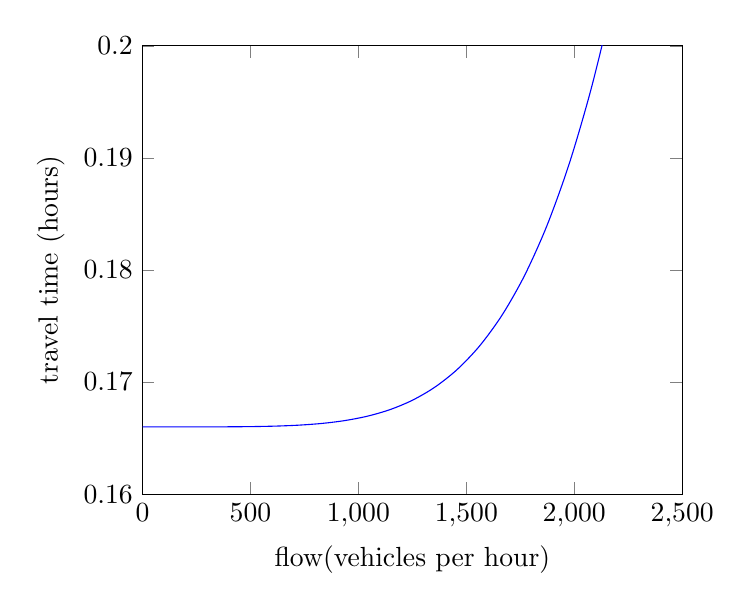
\begin{tikzpicture}
        \begin{axis}
            [
                domain=0:2500,
                black, no markers, smooth,
            %xtick=\empty, ytick=\empty,
                xlabel=flow(vehicles per hour), ylabel=travel time (hours),
                xmin=0,xmax=2500,
                ymin=0.16,ymax=0.2,
                yticklabel style={/pgf/number format/fixed, /pgf/number format/precision=3}
            ]
            \addplot {0.166*(1+0.15*(x/2000)^5)}; 
        \end{axis}
    \end{tikzpicture}
    \caption{Travel time function.}
    \label{fig:flowfunction}
\end{figure}
\marginpar{TODO\\correct\\diagram\\show\\zero flow}

Modifying Step 1 of the GSP for A*:
\begin{algorithm}
    \caption{A* Algorithm}
    \begin{algorithmic}[1]
        \Procedure{AStar}{$s, t$}
        \State $\mathcal{Q} \gets \{s\}$ \Comment{Add node $s$ with $d_s = h_s$}
        \State $p_s \gets -1$
        \State $d_s \gets 0$
        \ForAll {$ u \in \mathcal{V} : u \neq s $} \Comment{All nodes unvisited except the source}
            \State $d_u \gets \infty$
        \EndFor

        \While{ $\mathcal{Q} \neq \emptyset$ }
        \State $ u \gets \text{top}(Q) $ \Comment{Remove $u$ such that $d_u + h_u = \displaystyle\min_{v \in \mathcal{Q}} \{ d_v + h_v \} $}
            \State $ \mathcal{Q} \gets \mathcal{Q} \char`\\ \{u\} $
            \If{ $u = t$ }
                \State \text{Terminate Procedure}
            \EndIf
            \If{ $u \neq \text{zone} $}
            \ForAll {$v : (u, v) \in \mathcal{A}$} \Comment{For all outgoing arcs from $u$}
                    \If {$d_u + c_{vw} < d_v$}
                        \State $d_v \gets d_u + c_{vw}$
                        \State $p_v \gets u$
                        %\If {$v \notin \mathcal{Q}$} \Comment{Include node $v$ if unvisited}
                        \State $\mathcal{Q} \gets \mathcal{Q} \cup \{v\}$ \Comment{Add node $v$ with $d_v = d_u + c_{vw} + h_v$}
                        %\EndIf
                    \EndIf
                \EndFor
            \EndIf
        \EndWhile
        \EndProcedure
    \end{algorithmic}
\end{algorithm}

Results:

\begin{table}[H]
    \centering
    \begin{tabular}{lrr rrr rrr}
        Network        & Iterations & STL & Binary & Ternary & Binomial & Fibonacci & Pairing & Skew \\
        SiouxFalls     & 85           & 0.16 & 0.14 & 0.16 & 0.22  & 0.22  & 0.14  & 0.14            \\
        Anaheim        & 10           & 0.15 & 0.19 & 0.19 & 0.33  & 0.22  & 0.18  & 0.17            \\
        Barcelona      & 27           & 5.44 & 6.53 & 6.54 & 11.45 & 7.62  & 6.56  & 6.10            \\
        Winnipeg       & 128          & 19.49& 24.34& 24.86& 44.41 & 27.93 & 24.23 & 21.85           \\ 
        ChicagoSketch  & 26           & 38.92& 46.00   & 44.00   & 78.02 & 53.28 & 45.10 & 42.90       
    \end{tabular}
    \caption{A* Algorithm Result}
    \label{table:astarresult}
\end{table}

\begin{figure}
    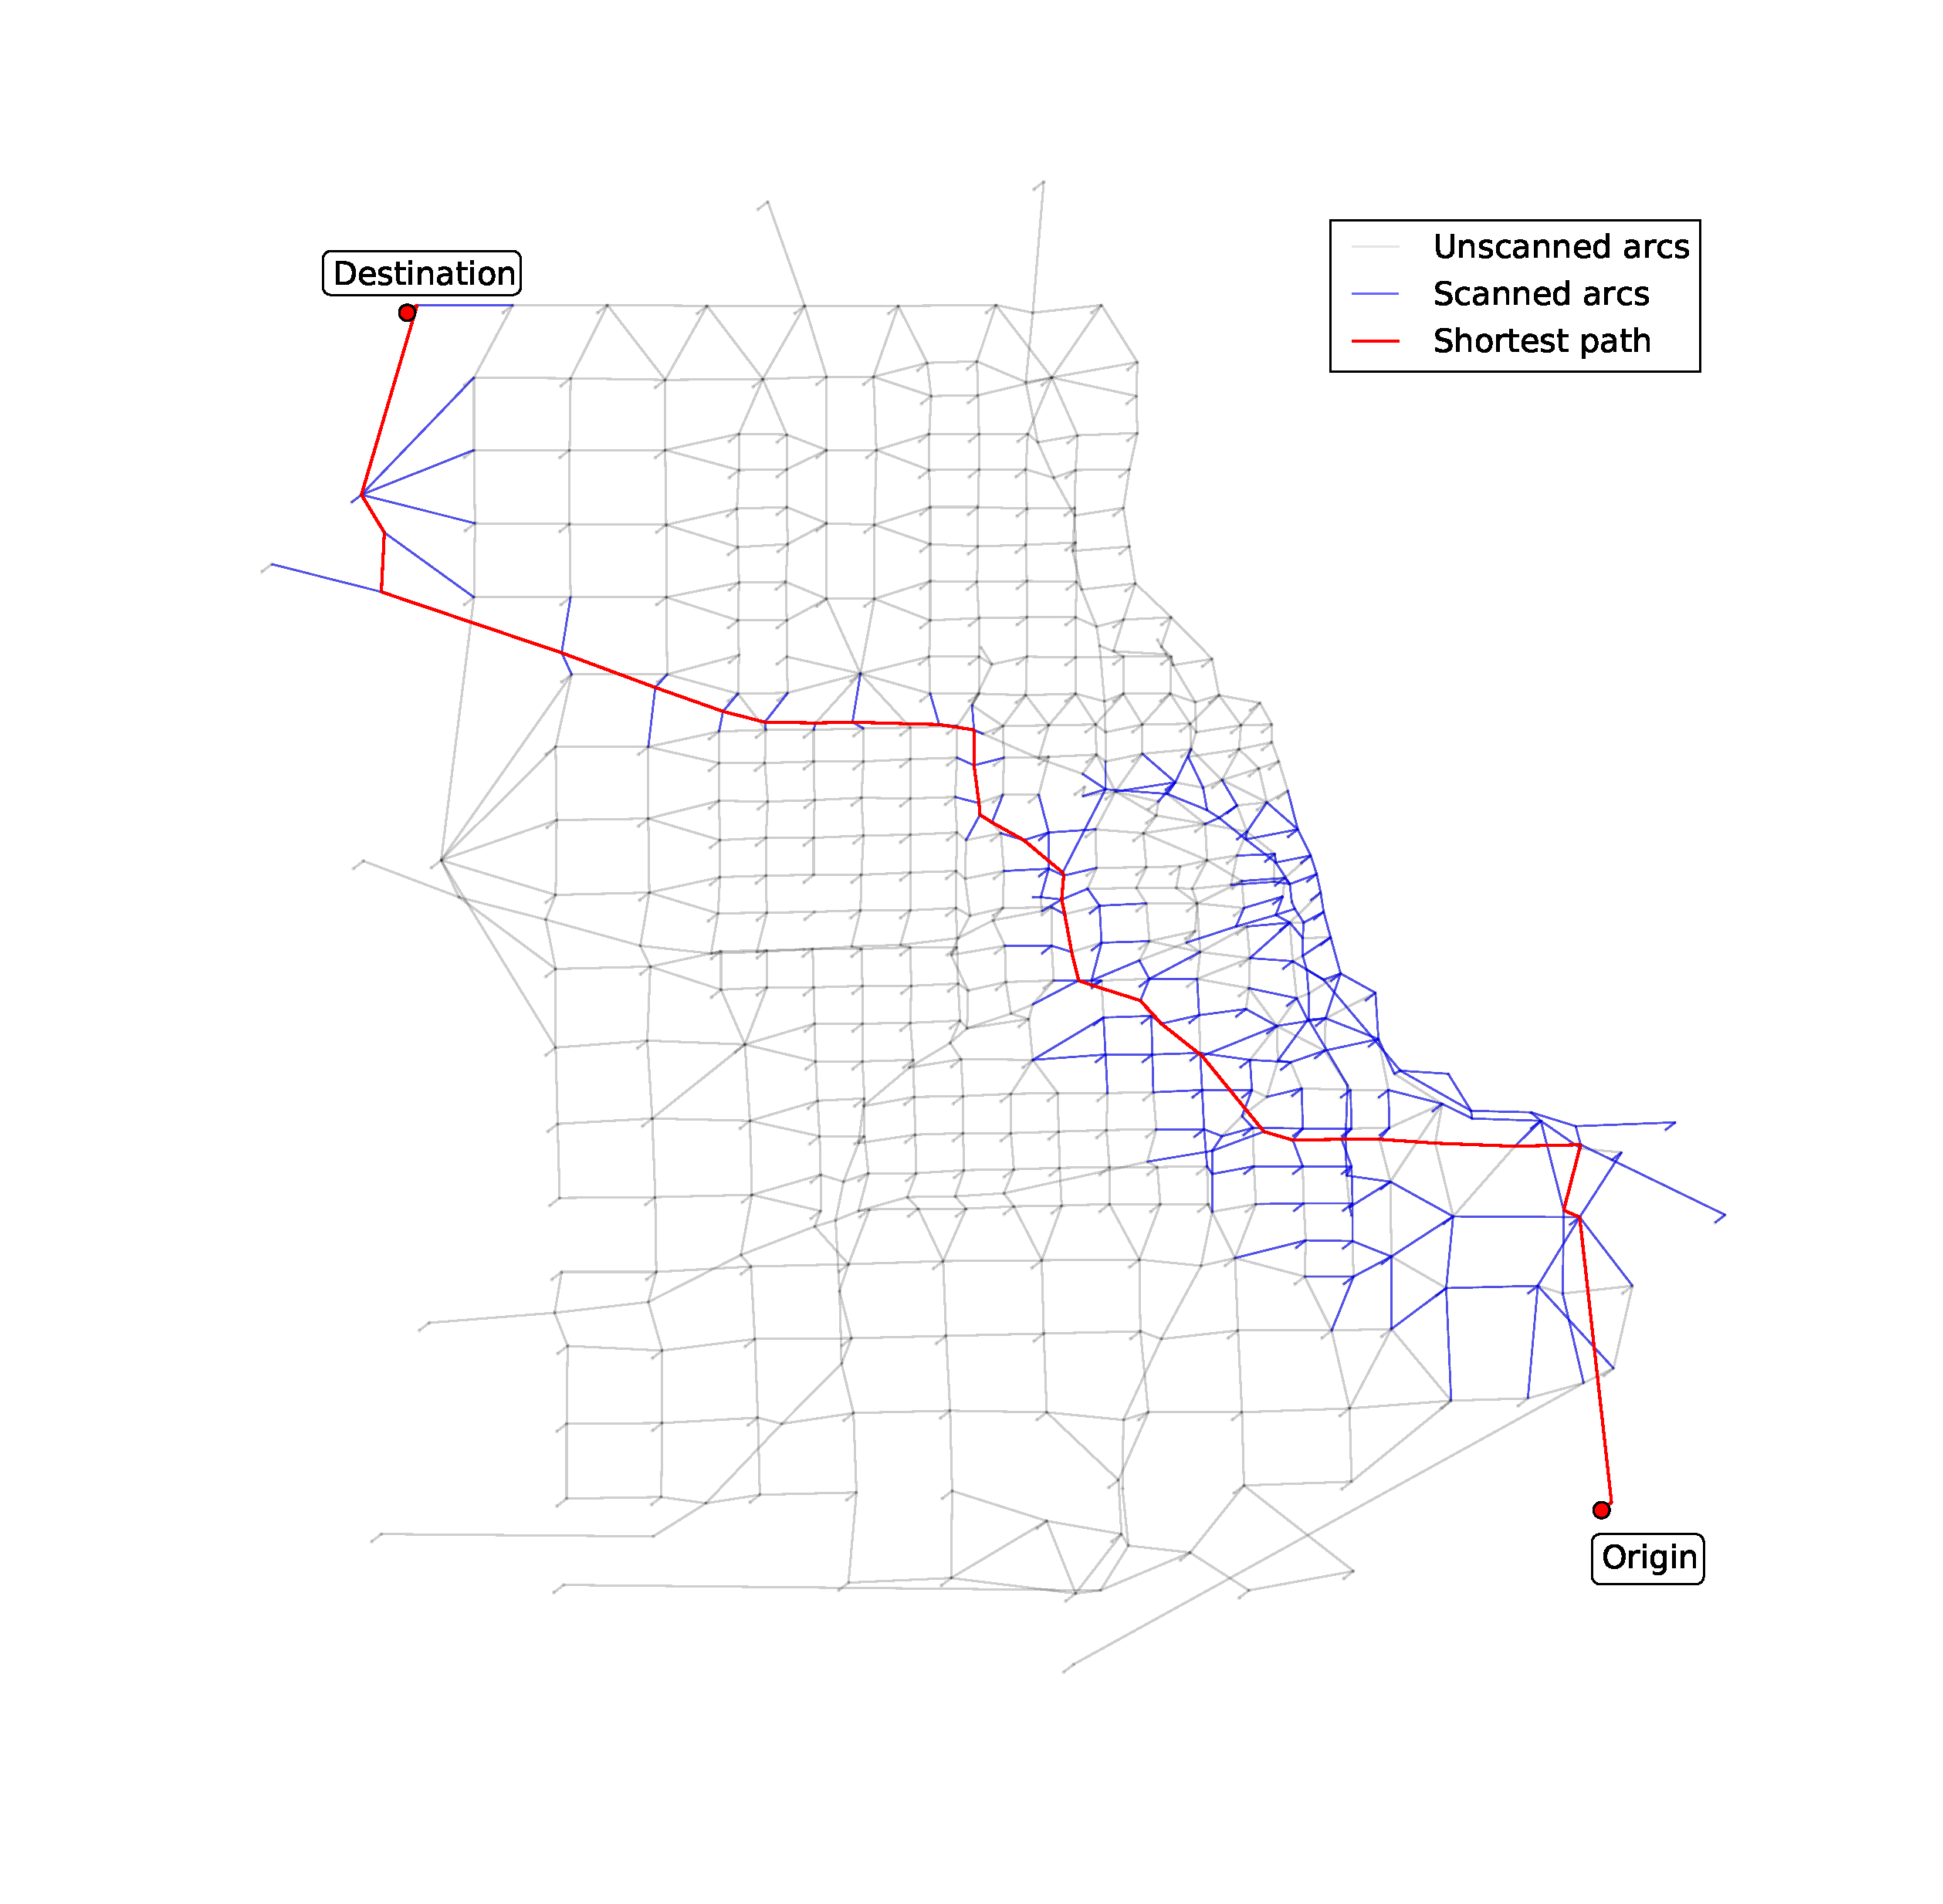
\includegraphics[width=\textwidth,trim=120px 120px 48px 120px,clip]{img/Astar_Chicago}
    \caption{A* Shortest Path Tree for ChicagoSketch network}
    \label{fig:astarchicago}
\end{figure}
Comparing the Dijkstra and A* algorithm's result (Table~\ref{table:dijkstraresult} and \ref{table:astarresult}),
we see an approximately 5 times improvement.
By looking at the shortest path tree generated
by the ChicagoSketch network,
there are only a few scanned nodes,
the path goes straight to the destination.
(TODO reference) says the closer the heuristic is to the actual
distance,
the better/faster shortest path calculation,
by looking at the travel time function (Figure~\ref{fig:flowfunction}, we can see the slope
is really shallow near the start,
and by comparing the initial flow and final flow (TODO, data),
\marginpar{TODO}
they are very close so the final flow is very close to the
initial flow,
which means the heuristic is a very good estimation,
which is our A* is very fast.

\section{Bidirectional A*}
\section{Preprocessing}
 

\newpage
\chapter{Computational Results}\label{chap:results}

This chapter shows the results from testing all the shortest path algorithms detailed in Chapter~\ref{chap:solvingspp} using the specific implementation described in the previous chapter.

The results are generated from using the g++ compiler using the -O3 optimise for speed option on Ubuntu 12.04 operating system, which has a Intel Core i5-3317U CPU with 3.8GiB RAM.

\section{Problem Data and Result Explanation}
The problem data for solving the TA problems are retrieved from Transportation Network Test Problems \citep{ProblemData}.
Table~\ref{table:problemdata} shows the data that are going to be tested with,
where the network name, numbers nodes, traffic analysis, origin-desitination (OD) pairs and edges are given.
\begin{table}[H]
    \centering
    \begin{tabular}{lrrrr} \toprule
        Network & Nodes & Zones & OD pairs & Edges \\ \cmidrule(lr){1-5}
        SiouxFalls    & 24   & 24  & 528   & 76   \\
        Anaheim       & 416  & 38  & 1406  & 914  \\
        Barcelona     & 1020 & 110 & 7922  & 2522 \\
        Winnipeg      & 1052 & 147 & 4344  & 2836 \\
        ChicagoSketch & 933  & 387 & 93135 & 2950 \\ \bottomrule
    \end{tabular}
    \caption{Network Problem Data}
    \label{table:problemdata}
\end{table}
\todo{the number of nodes listed in the table includes traffic zones}
By examining the network problem data,
we can see that the number of OD pairs increase
significantly respect to the number of zone nodes,
this is important because it indicates how many point to point SPPs need to be solved for each iteration of the PE method.
We can also roughly tell that these networks are very sparse;
for a complete graph (every node is connected to every other node) of 1000 nodes have 499500 edges ($n(n-1)/2$),
but the larger networks in our problem data only have about 0.4\% to 0.6\% of edges in the corresponding complete graph. 
Analysing the graph shows the degree of any vertex in the graph is no more than 5.
This information is useful
for choosing the best algorithm and data structure.

The correctness of the final shortest path trees are checked by comparing to the label correcting algorithm that is implemented by the co-supervisor of this project, which is guarantee to be correct.

\section{Discussion of Computational Results}
In Table~\ref{table:allresults} we present the running times for a complete run of the Traffic Assignment Path Equilibration method.
For each network, each of the algorithms
\begin{itemize}
    \item label correcting Bellman-Ford (B),
    \item one source Dijkstra (1S-D),
    \item point to point Dijkstra (P2P-D),
    \item bidirectional Dijkstra (Bi-D),
    \item A* search (A*),
    \item bidirectional A* search (Bi-A*),
\end{itemize}
is used for each of the networks shown in Table~\ref{table:problemdata}.
The numbers of iterations (ITERS) each algorithm took,
The overall number of nodes scanned in the network (COUNT),
and the total run time (seconds) each algorithm took is shown.
Each algorithm is also compared to the label correcting algorithm to show the percentage speed-up (SPD).

\begin{table}
    \centering
    \begin{tabular}{l l r rr rr } \toprule
        & & & \multicolumn{2}{c}{Max Scans} & \multicolumn{2}{c}{Time} \\ 
        \cmidrule(lr){4-5}
        \cmidrule(lr){6-7}
        Network & Algorithm & ITERS & COUNT & SPD                     & SEC & SPD \\ 
        \cmidrule(lr){1-1}
        \cmidrule(lr){2-2}
        \cmidrule(lr){3-3}
        \cmidrule(lr){4-4}
        \cmidrule(lr){5-5}
        \cmidrule(lr){6-6}
        \cmidrule(lr){7-7}
        SiouxFalls    & B     & 69 & & & 0.25 & \\
        & 1S-D  & 69 & & & 0.24 & \\
        & P2P-D & 64 & & & 0.15 & \\
        & Bi-D  & & & & & \\
        & A*    & 85 & & & 0.16 & \\
        & Bi-A* & & & & & \\ \\
        Anaheim       & B     & 10 & & & 1.20 & \\
        & 1S-D  & 10 & & & 1.20 & \\
        & P2P-D & 10 & & & 0.67 & \\
        & Bi-D  & & & & & \\
        & A*    & 10 & & & 0.15 & \\
        & Bi-A* & & & & & \\ \\
        Barcelona     & B     & 28 & & & 60.00 & \\
        & 1S-D  & 28 & & & 43.00 & \\
        & P2P-D & 27 & & & 27.71 & \\
        & Bi-D  & & & & & \\
        & A*    & 27 & & &  6.10 & \\
        & Bi-A* & & & & & \\ \\
        Winnipeg      & B     & 129 & & & 190.00 & \\
        & 1S-D  & 129 & & & 137.00 & \\
        & P2P-D & 129 & & &  70.00 & \\
        & Bi-D  & & & & & \\
        & A*    & 128 & & & 21.85 & \\
        & Bi-A* & & & & & \\ \\
        ChicagoSketch & B     & 25 & & & 500.00 & \\
        & 1S-D  & 25 & & & 541.00 & \\
        & P2P-D & 25 & & & 204.00 & \\
        & Bi-D  & & & & & \\
        & A*    & 26 & & & 42.90 & \\
        & Bi-A* & & & & & \\
        \bottomrule
    \end{tabular}
    \caption{Results for all test networks. Showing the number of iterations for each network (ITERS), max number of scans (COUNT) and the speed up respect to the label correcting algorithm (SPD). }
    \label{table:allresults}
\end{table}
\todo[noline]{Result : average number of scans}
\todo[inline]{Result table for all heaps}

Figure~\ref{fig:long_sptree} shows the shortest path tree between two distant nodes in the ChicagoSketch network.
We can see Dijkstra's algorithm scans the whole network.
Bidirectional Dijkstra scans almost the whole network with a few nodes not being scanned.
A* search scans only a small region of the network.
\todo{incomplete}
\begin{figure}
    \centering
    \begin{subfigure}{.5\textwidth}
        \centering
        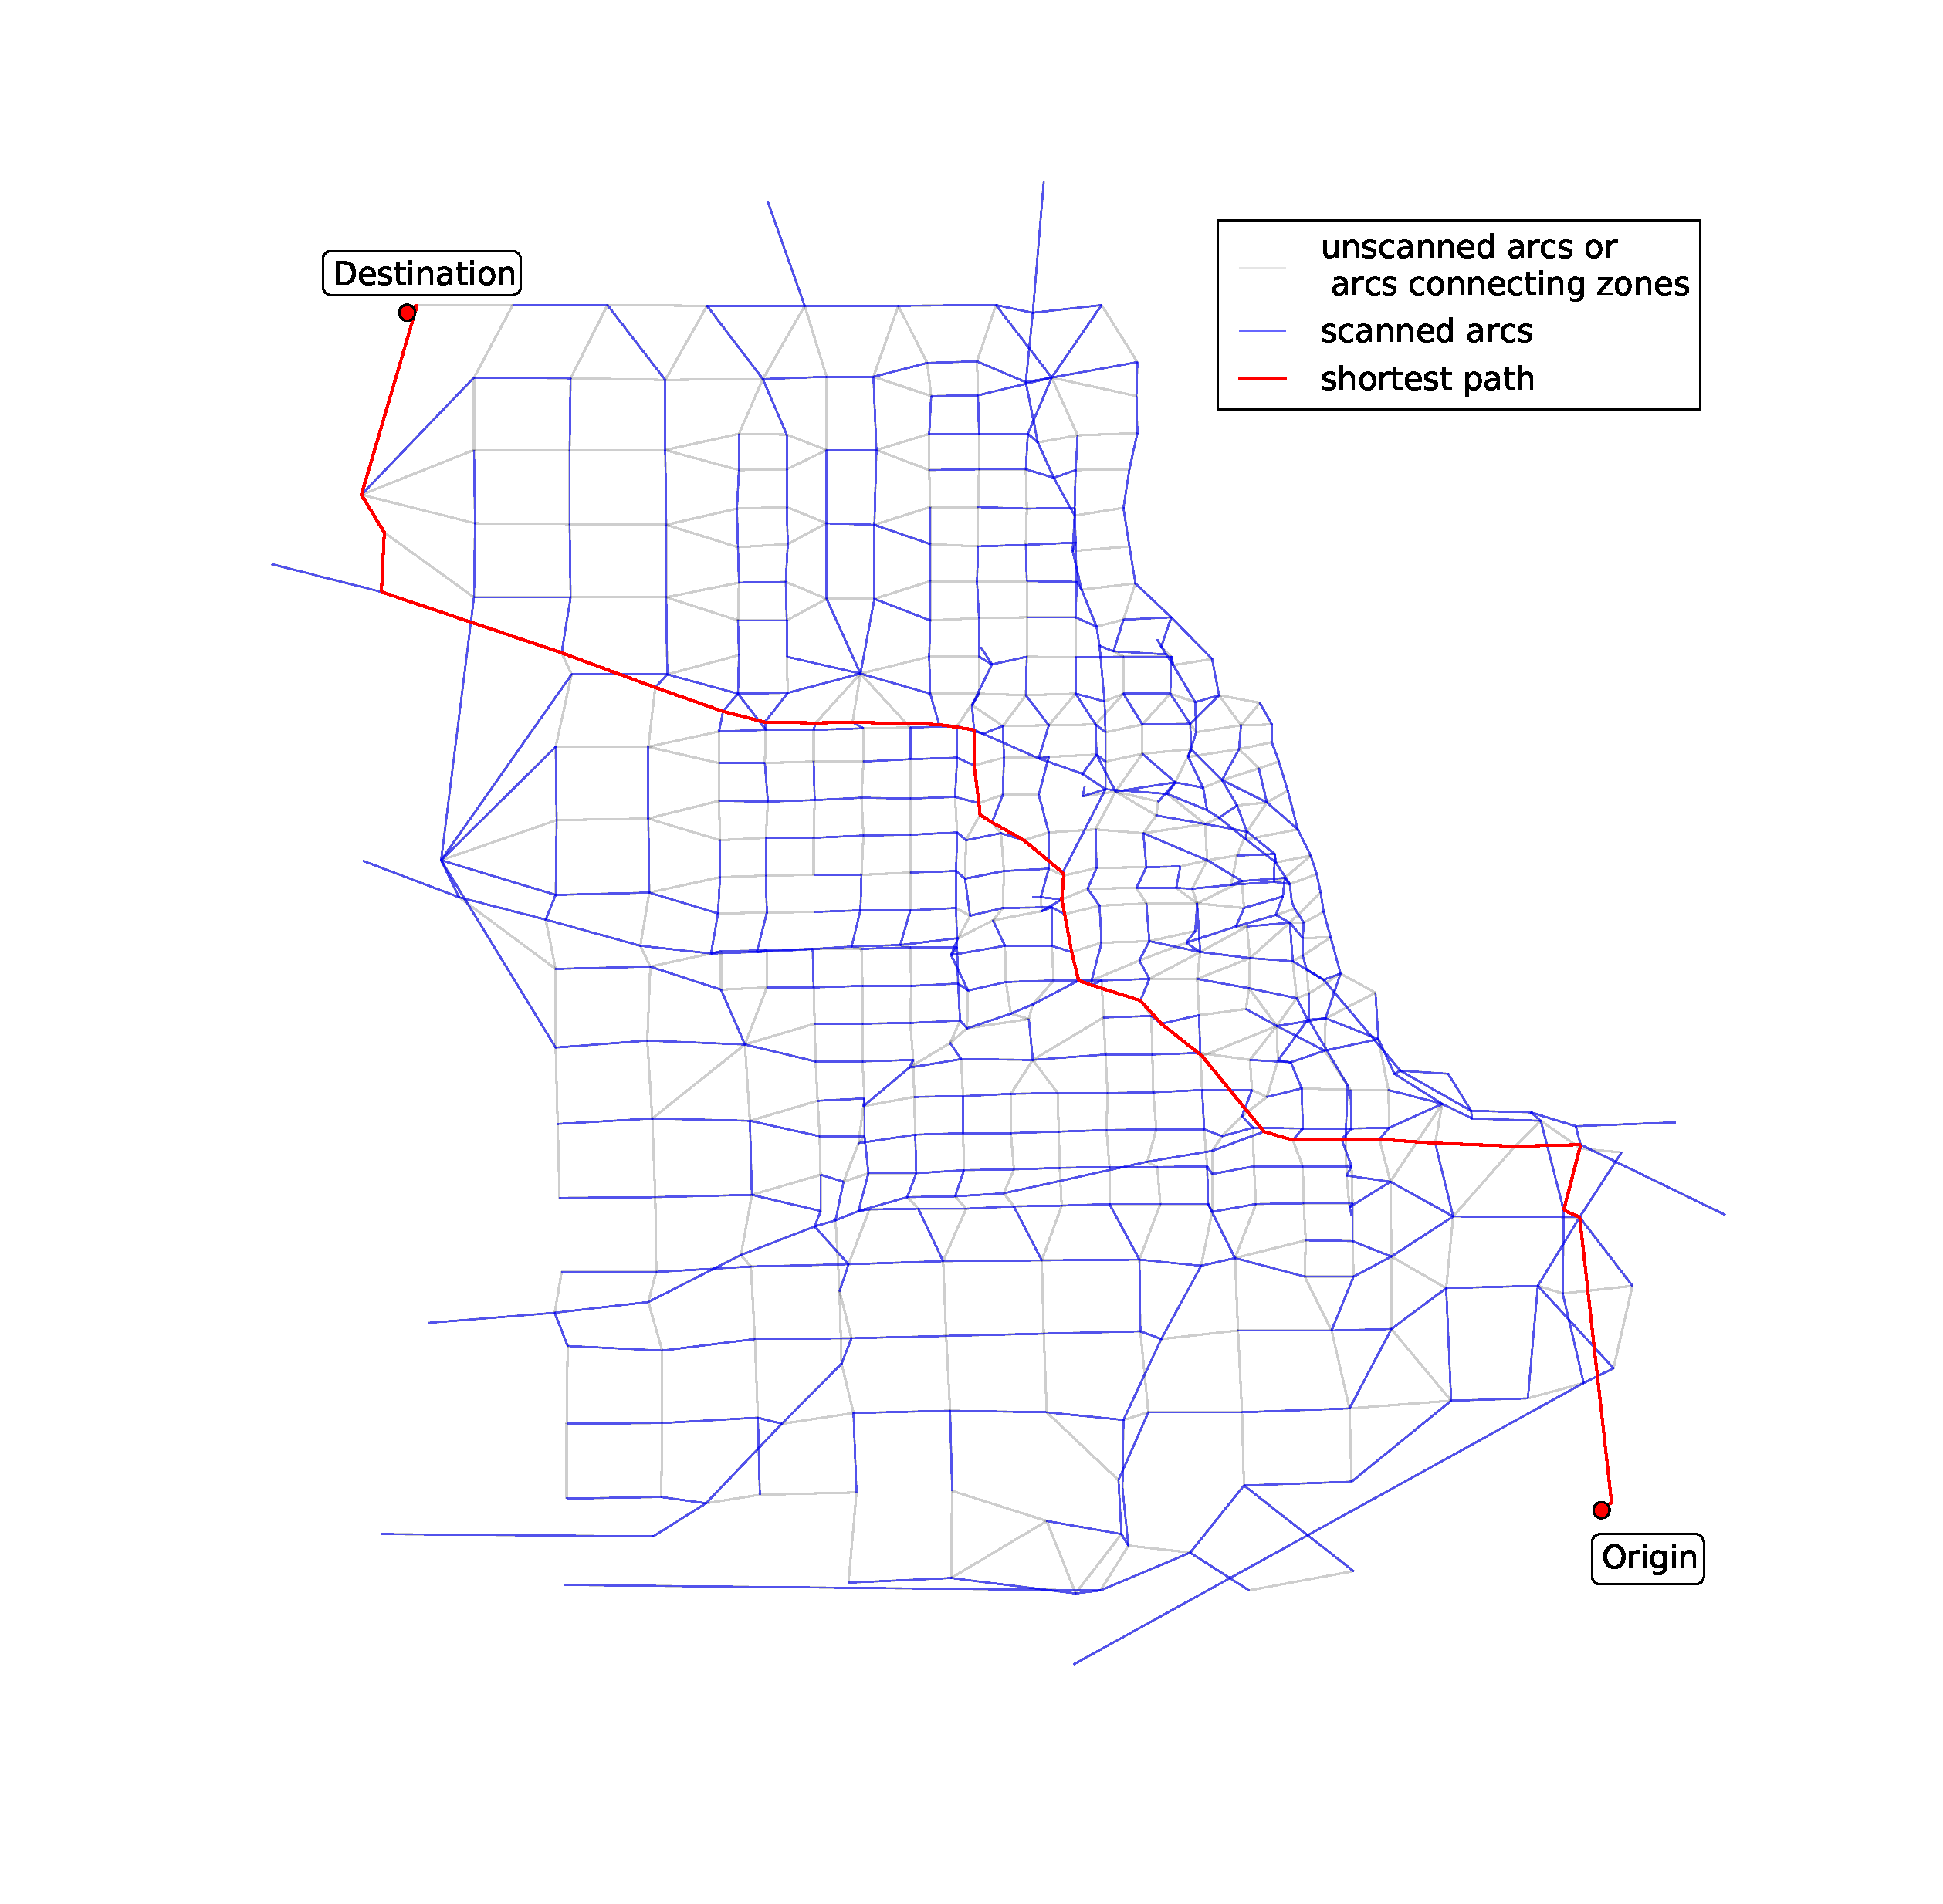
\includegraphics[width=\textwidth,trim=120px 120px 48px 120px,clip]{img/chicago_dijkstra}
        \caption{Dijkstra}
        \label{fig:chicago_dijkstra}
    \end{subfigure}%
    \begin{subfigure}{.5\textwidth}
        \centering
        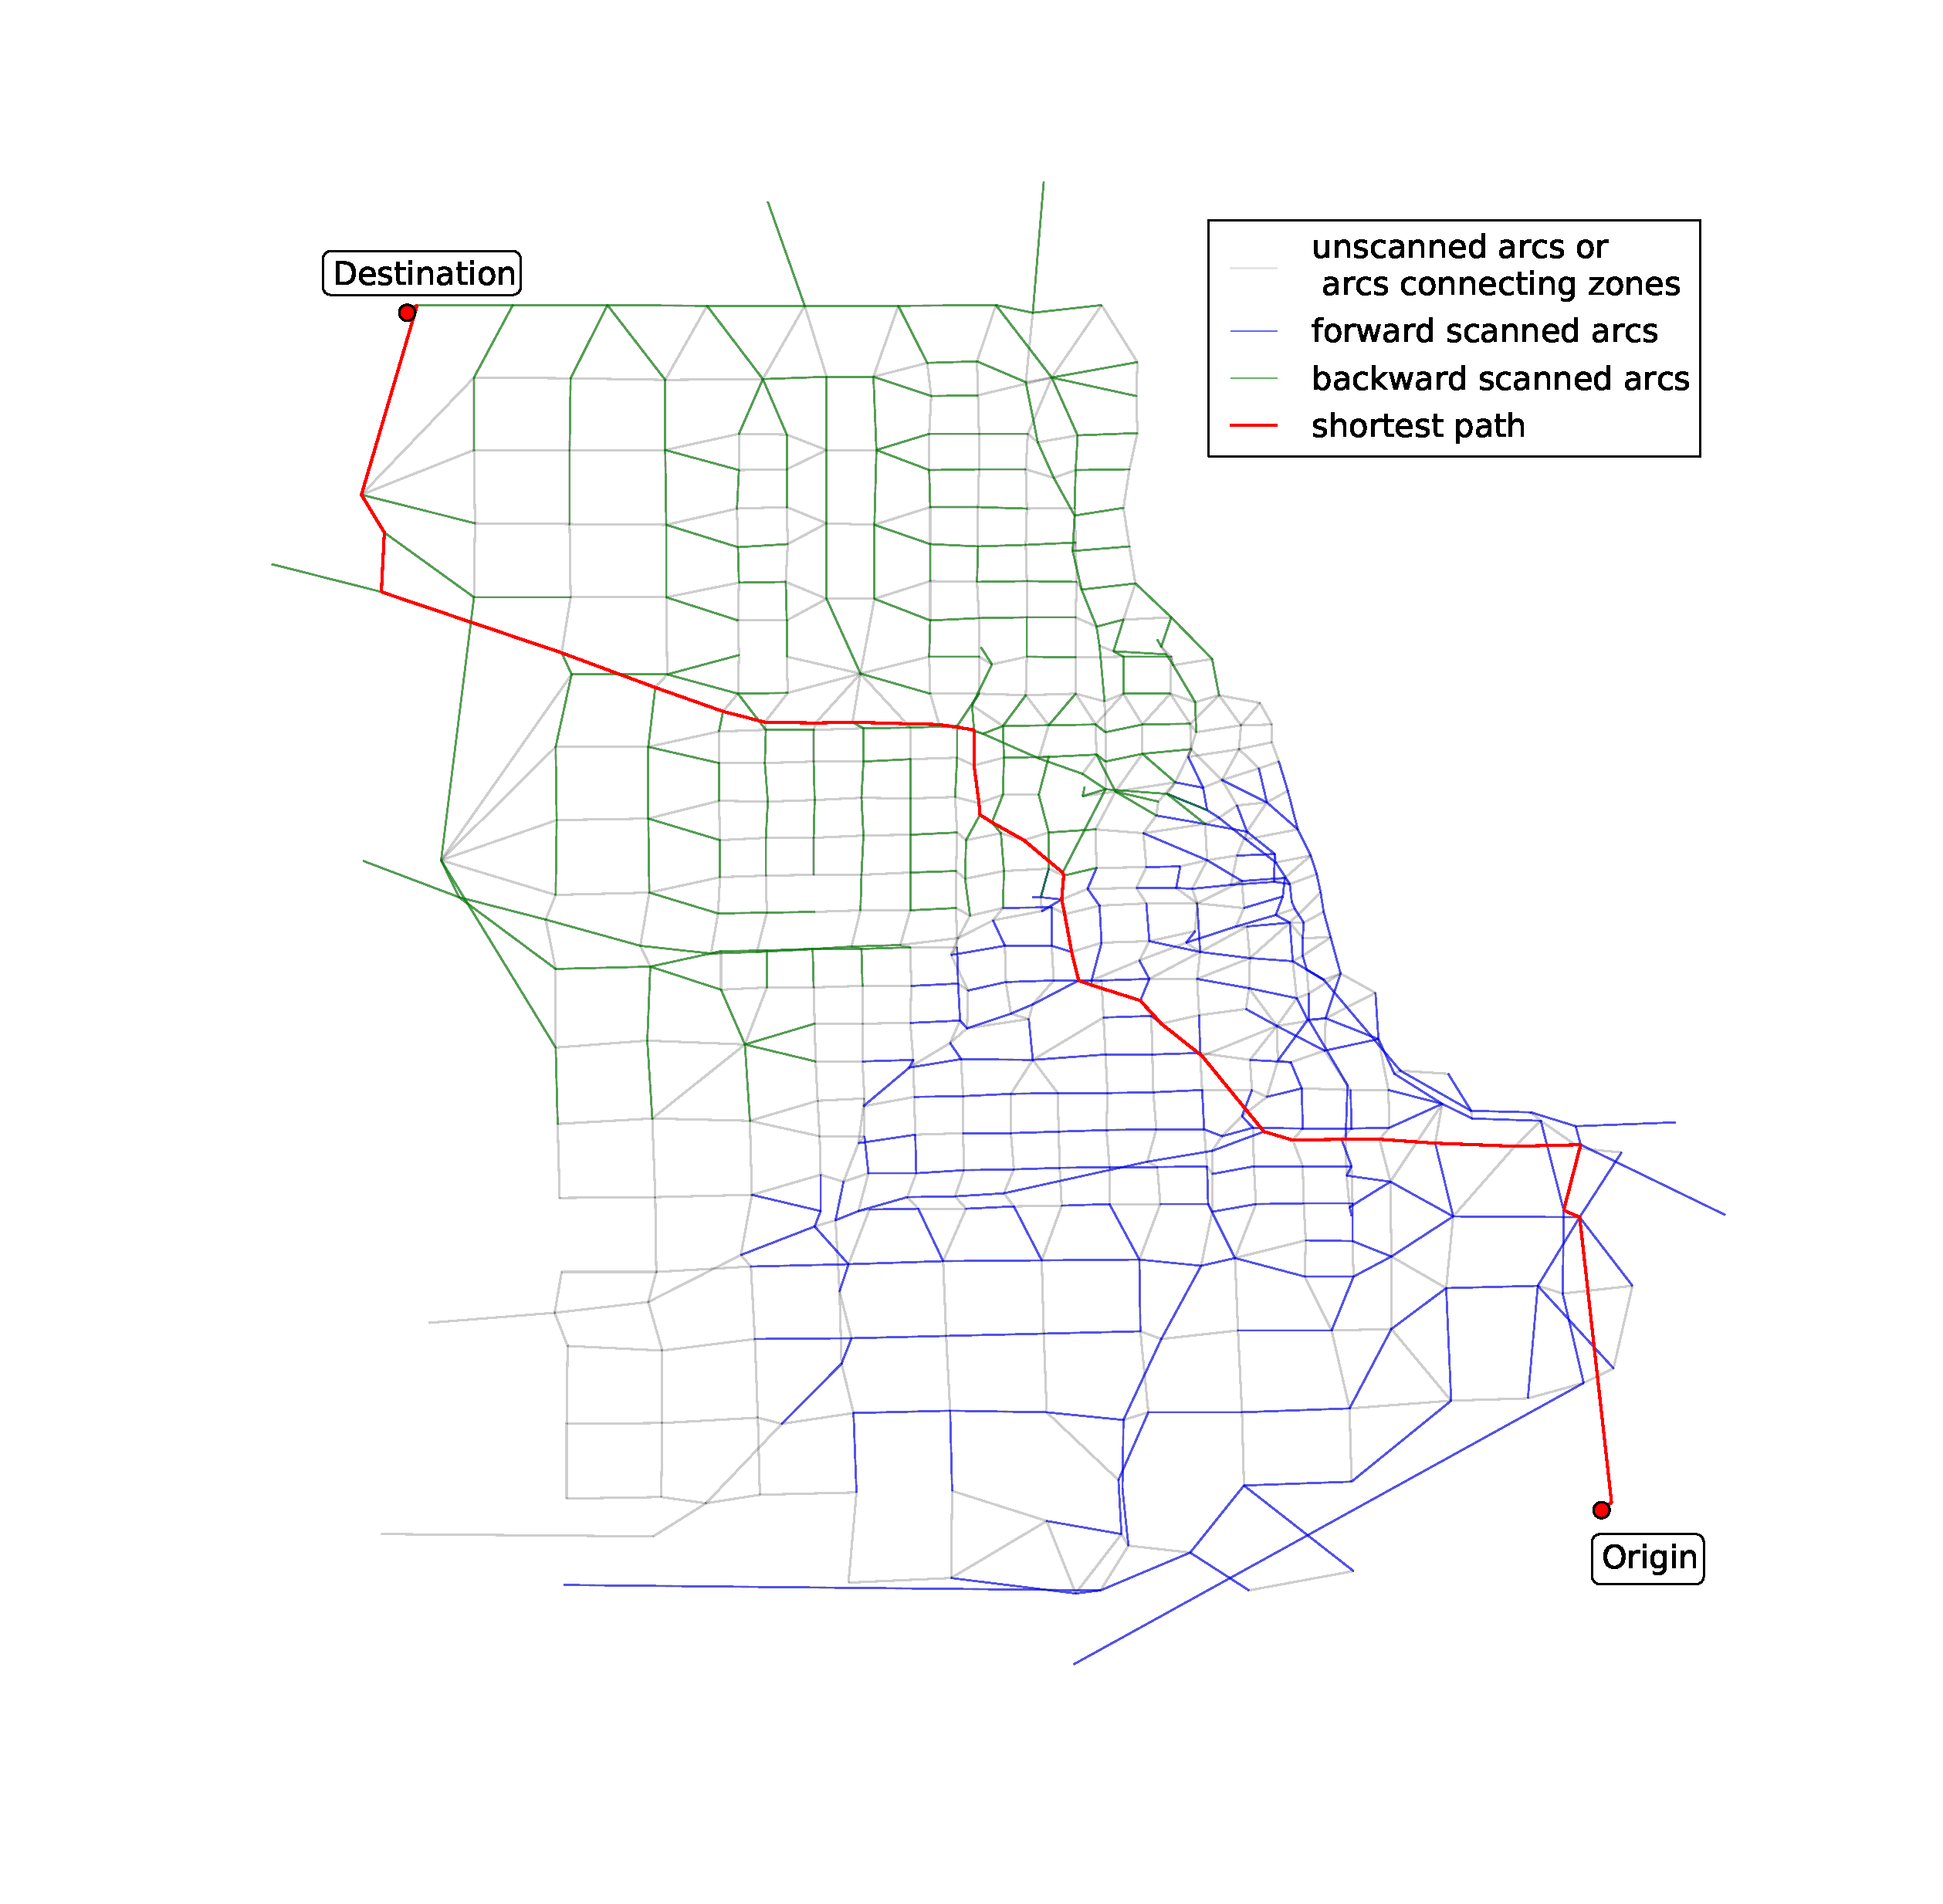
\includegraphics[width=\textwidth,trim=120px 120px 48px 120px,clip]{img/chicago_bidirect}
        \caption{Bidirectional Dijkstra}
        \label{fig:chicago_bidirect}
    \end{subfigure}
    \begin{subfigure}{.5\textwidth}
        \centering
        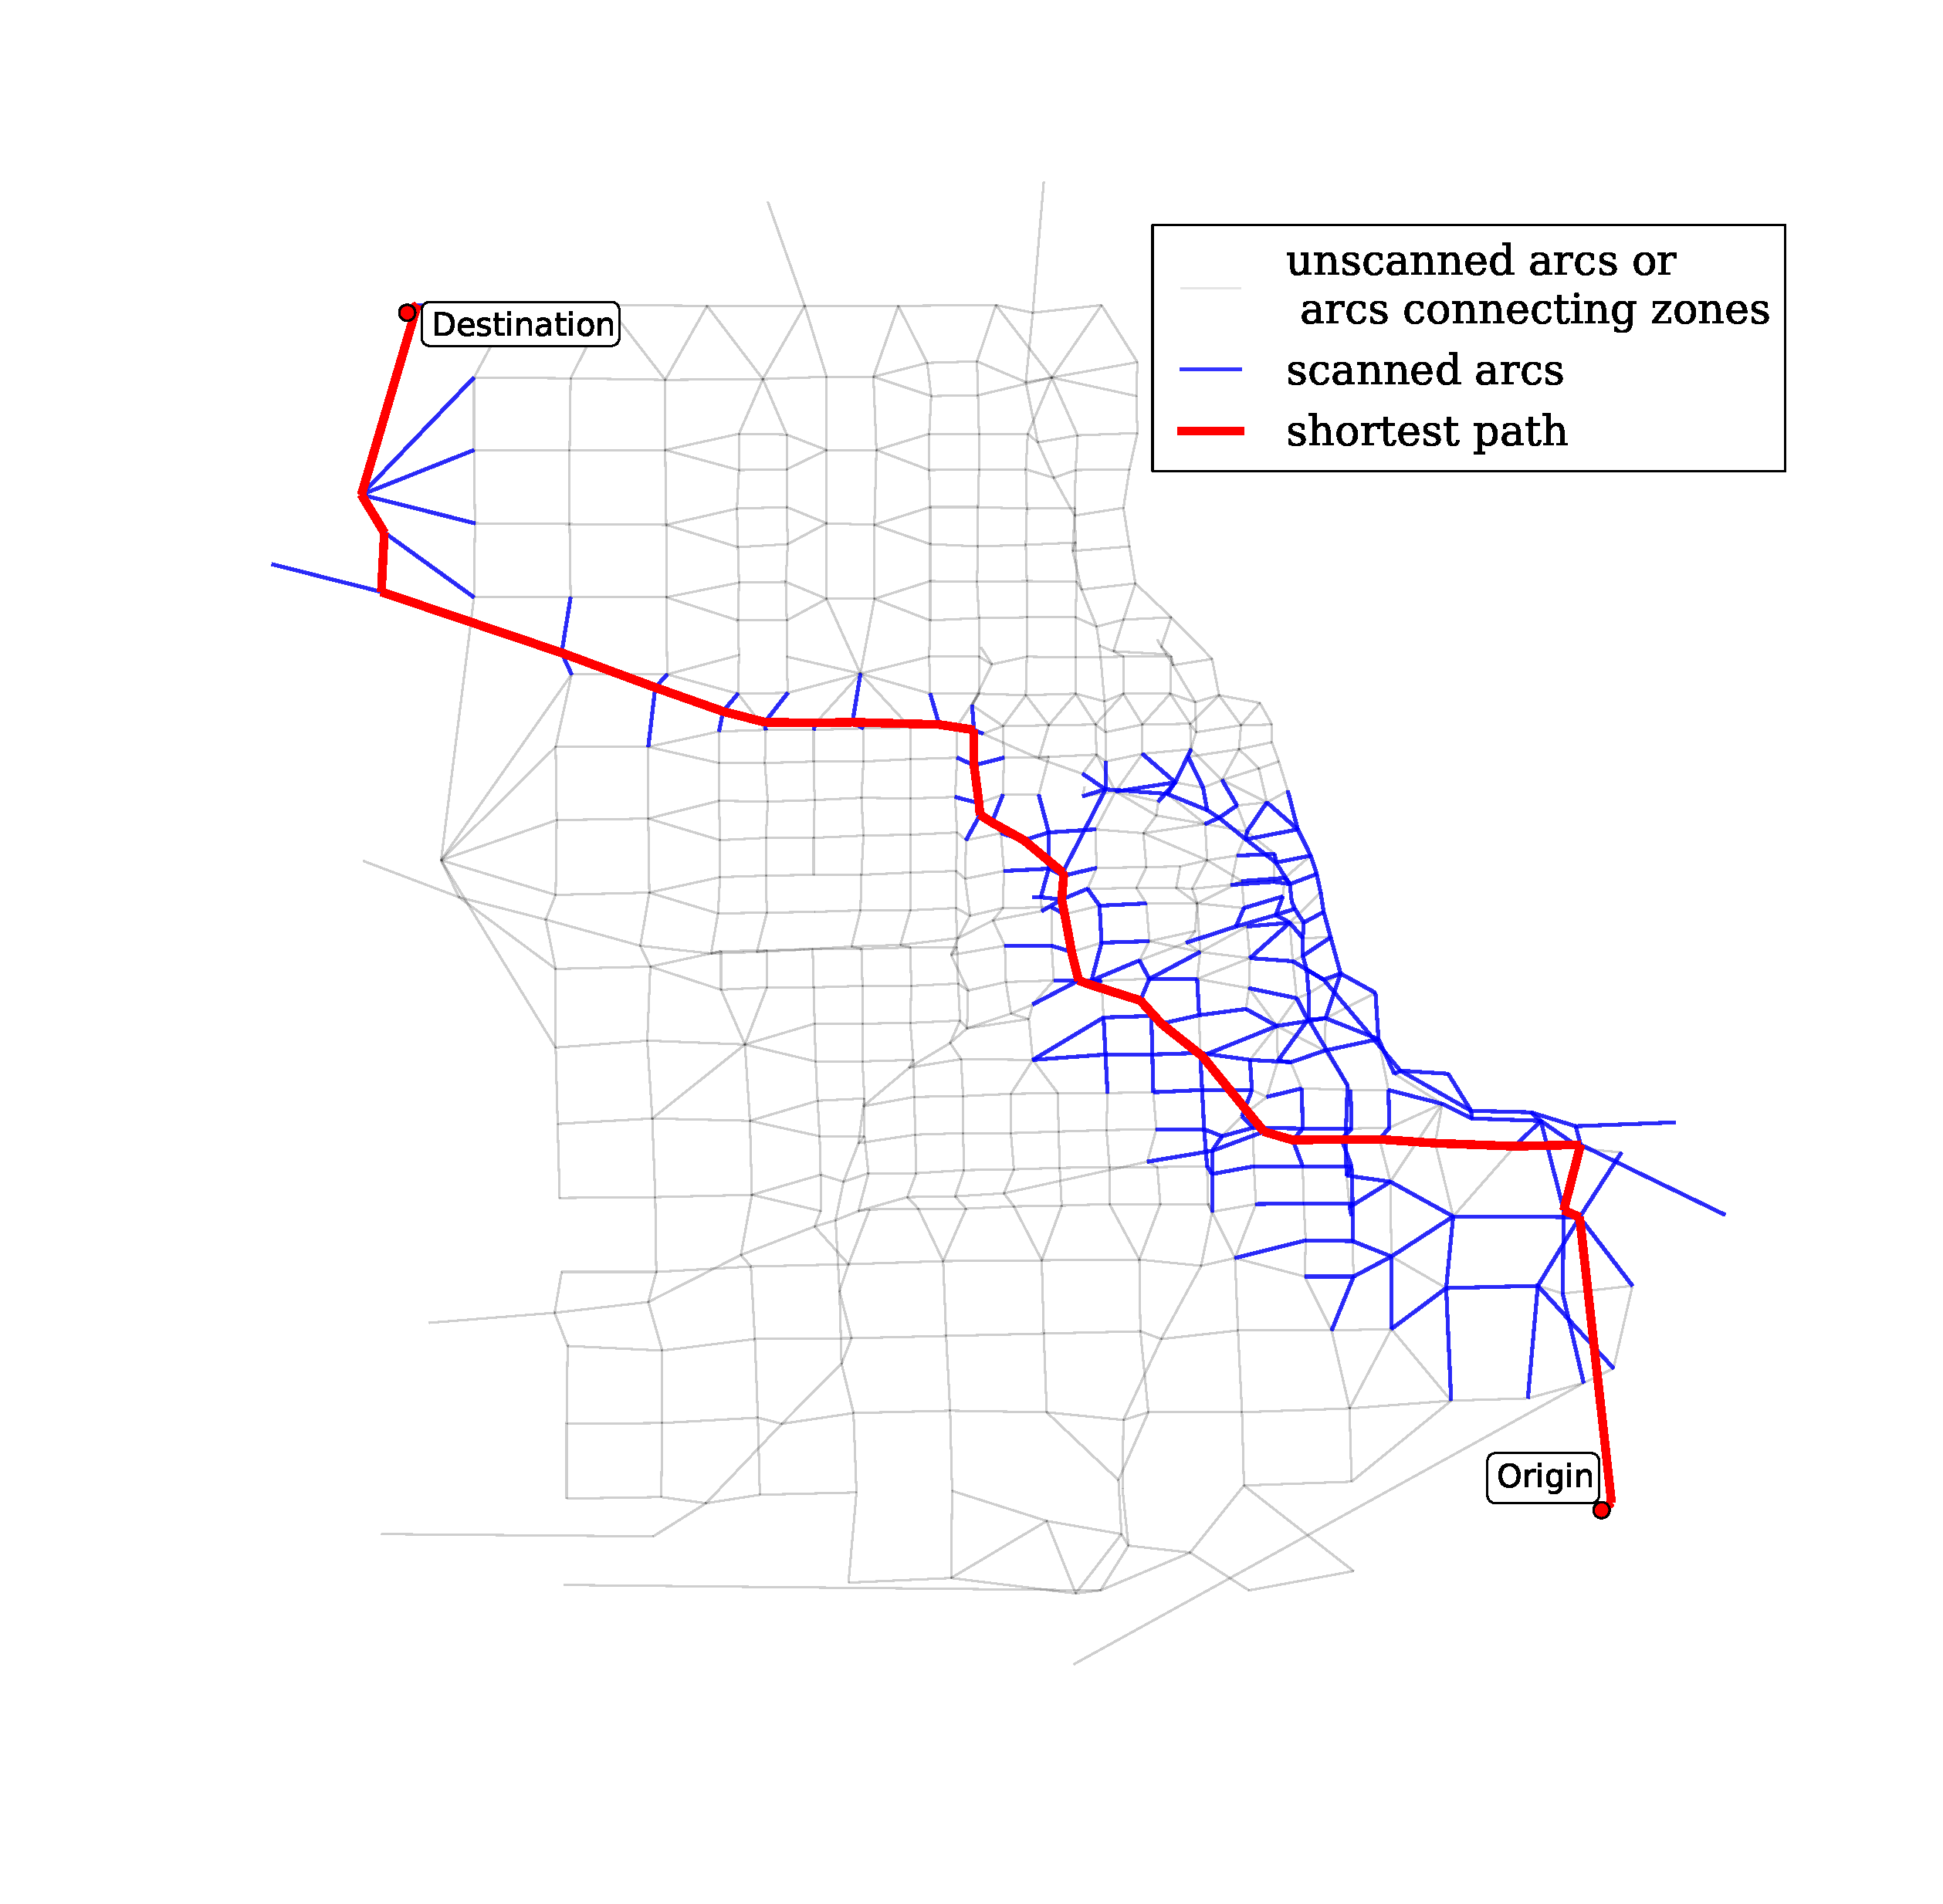
\includegraphics[width=\textwidth,trim=120px 120px 48px 0px,clip]{img/chicago_astar}
        \caption{A* Search}
        \label{fig:chicago_Astar_bidirect}
    \end{subfigure}%
    \begin{subfigure}{.5\textwidth}
        \centering
        \missingfigure[figwidth=\textwidth]{Bidirectional A*}
    %    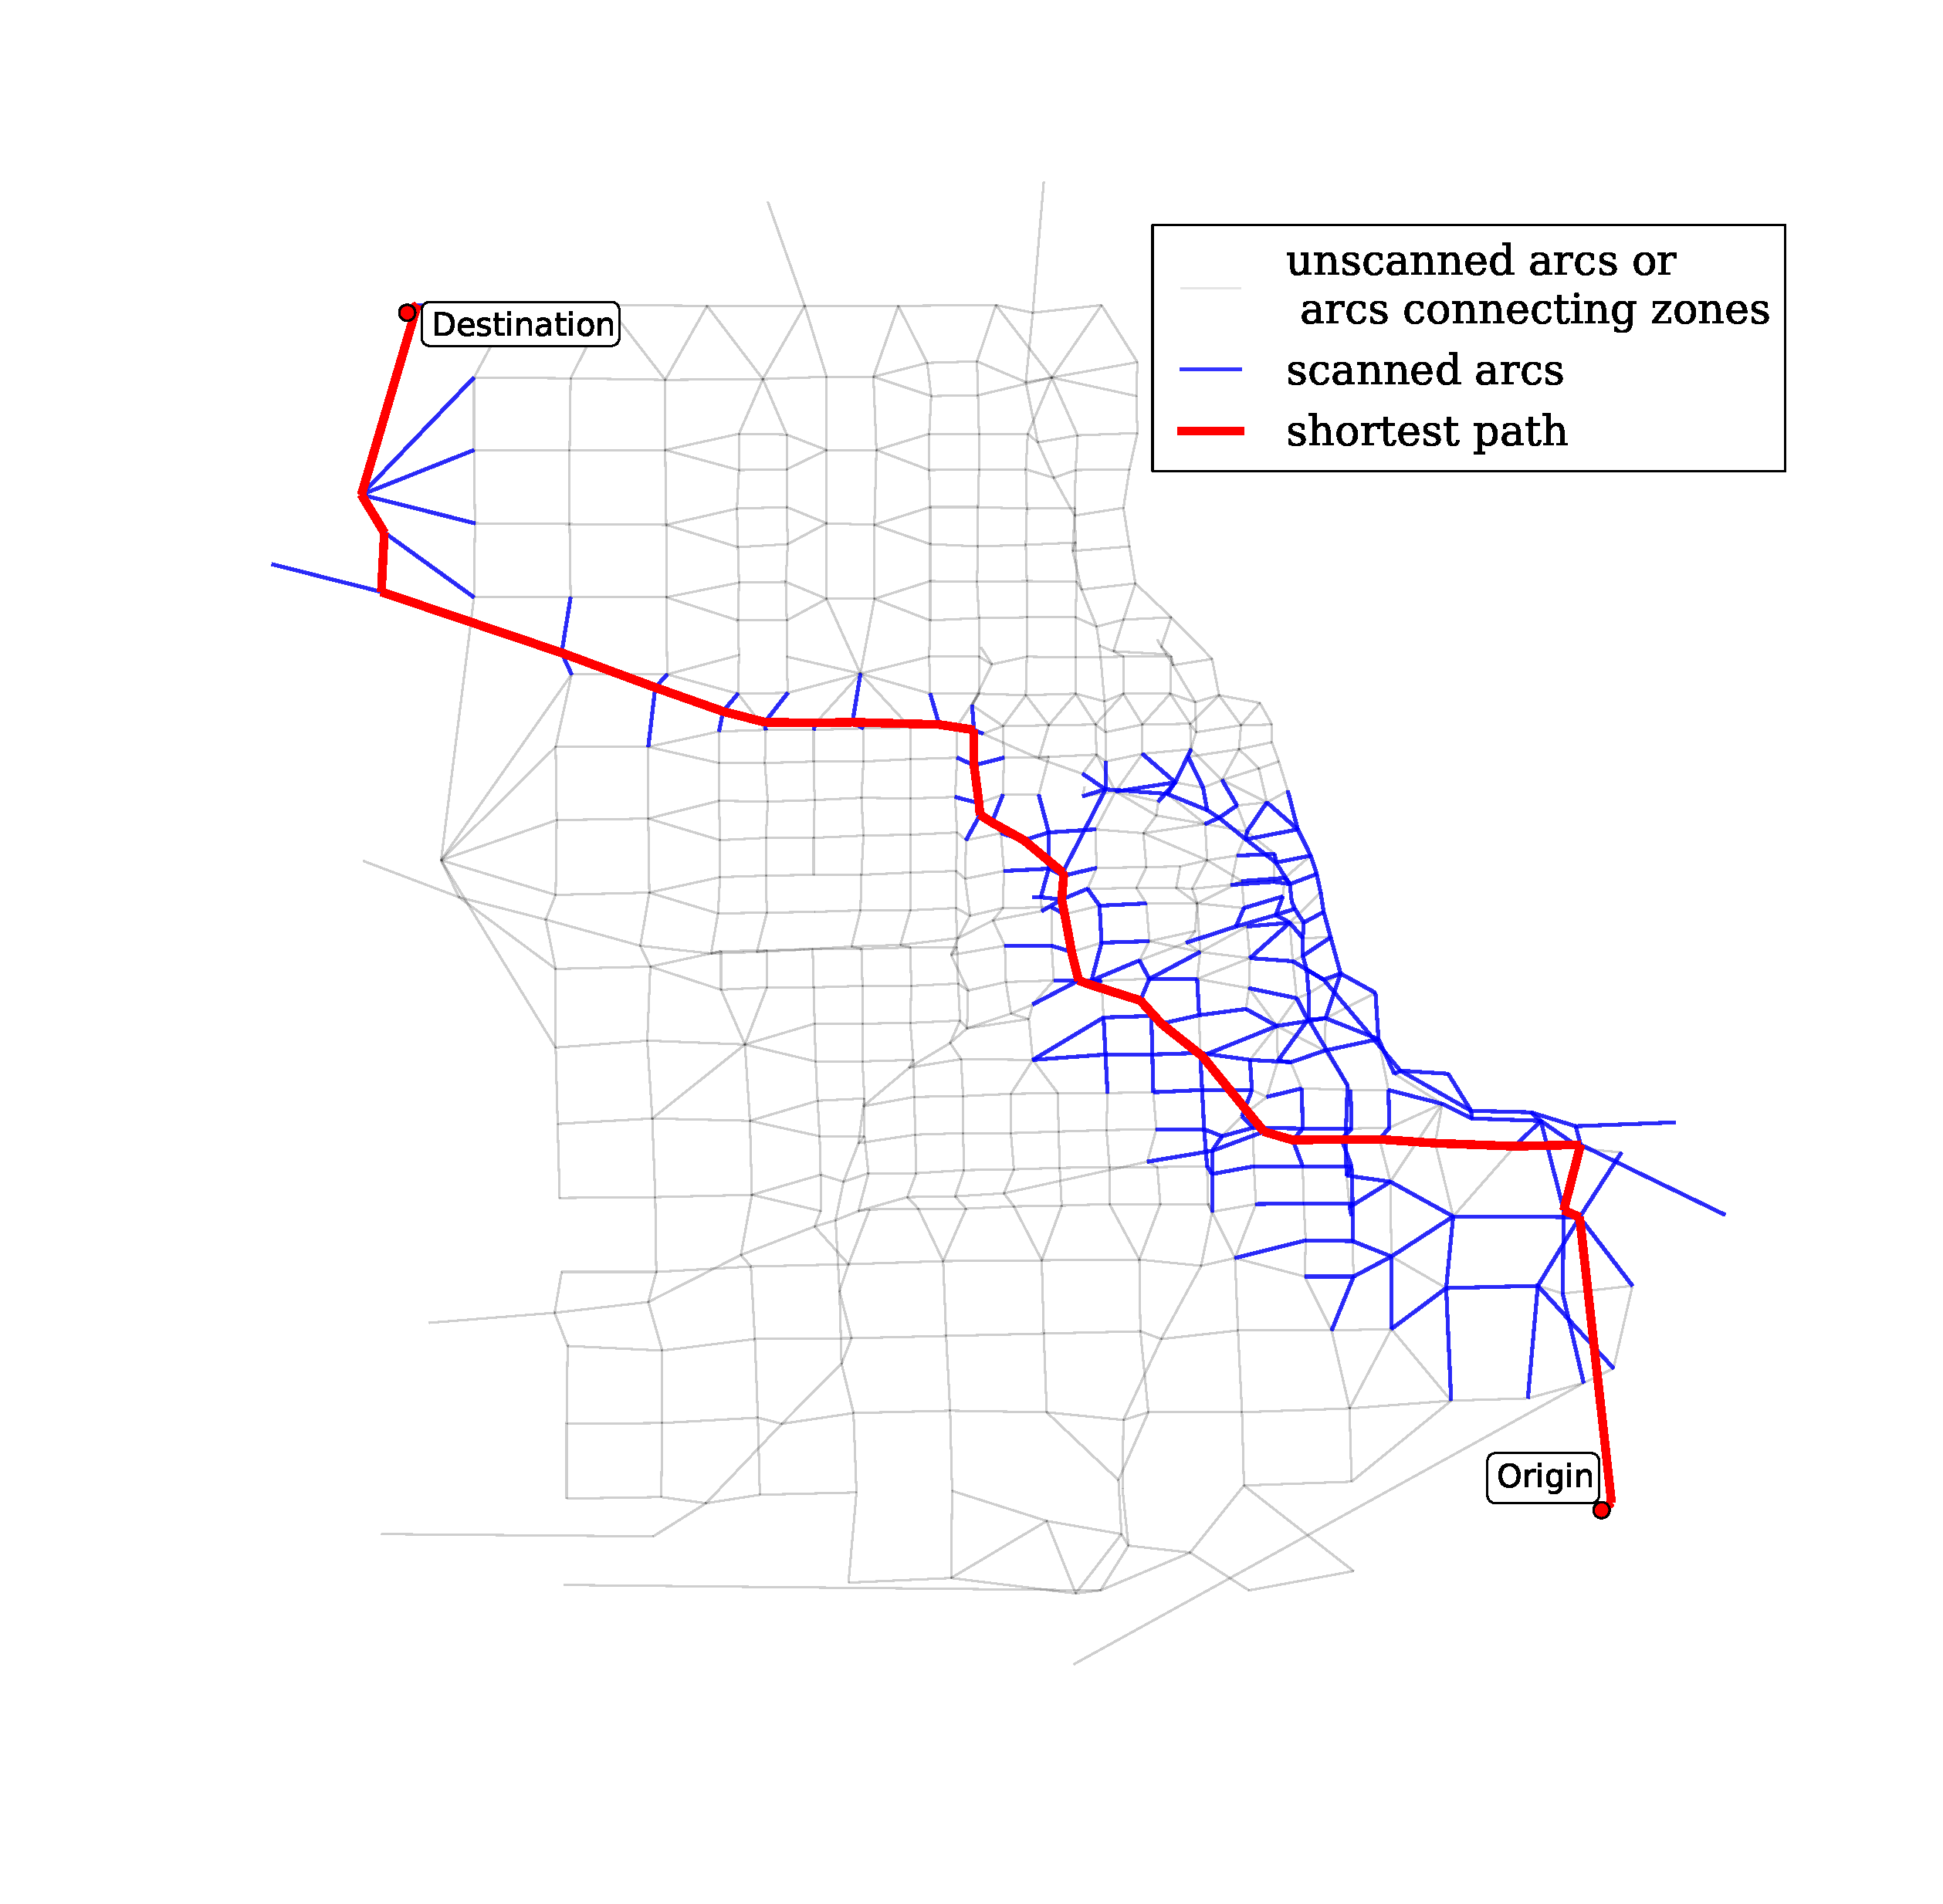
\includegraphics[width=\textwidth,trim=120px 120px 48px 0px,clip]{img/chicago_astar}
        \caption{Bidirectional A* Search}
        \label{fig:chicago_astar_bidirect}
    \end{subfigure}
    \vspace{1em}
    \caption{Shortest Path Tree between Two Distant Nodes in the ChicagoSketch Network -D Pair}
    \label{fig:long_sptree}
\end{figure}
\todoin{draw 2 nodes that are close to each other}


\begin{comment}

All of these run times are slower than the STL version of the Heap.
Upon inspection,
it is found that the increase-key operation is used about between 5\% to 10\%
of the time,
\todo{not actual count yet}
which means the graphs are not dense enough for these Heap structures to outperform a
simple array based priority queue.
Comparing the Dijkstra and A* search algorithm's result,
we see an approximately 5 times improvement.
By looking at the shortest path tree generated
by the ChicagoSketch network,
there are only a few scanned nodes,
the path goes straight to the destination.
(TODO reference) says the closer the heuristic is to the actual distance,
the better/faster shortest path calculation,
by looking at the travel time function (Figure~\ref{fig:flowfunction}, we can see the slope
is really shallow near the start,
and by comparing the initial flow and final flow (TODO, data),
they are very close so the final flow is very close to the
initial flow,
which means the heuristic is a very good estimation,
which is our A* search is very fast.
\end{comment}


\todo[inline]{give results interpretation}


\newpage
\chapter{Conclusions} \label{chap:conclusions}
A* search out performs all other algorithms \ldots



\newpage
%\appendix
%\begin{appendices}
%\end{appendices}


\newpage
\bibliographystyle{agsm}
\renewcommand{\bibname}{References}
\bibliography{citations}

\end{document}
